\documentclass[11pt]{elegantbook}
\definecolor{structurecolor}{RGB}{40,58,129}
\linespread{1.6}
\setlength{\footskip}{20pt}
\setlength{\parindent}{0pt}
\newcommand{\argmax}{\operatornamewithlimits{argmax}}
\newcommand{\argmin}{\operatornamewithlimits{argmin}}
\elegantnewtheorem{proof}{Proof}{}{Proof}
\elegantnewtheorem{claim}{Claim}{prostyle}{Claim}
\DeclareMathOperator{\col}{col}
\title{\textbf{Useful Economic Theory and Mathematics}}
\author{Wenxiao Yang}
\institute{Haas School of Business, University of California Berkeley}
\date{2023}
\setcounter{tocdepth}{2}
\cover{cover.png}
\extrainfo{All models are wrong, but some are useful.}

% modify the color in the middle of titlepage
\definecolor{customcolor}{RGB}{9,119,119}
\colorlet{coverlinecolor}{customcolor}
\usepackage{cprotect}

\addbibresource[location=local]{reference.bib} % bib

\begin{document}

\maketitle
\frontmatter
\tableofcontents
\mainmatter



\chapter{Stochastic Dominance}
Based on
\begin{enumerate}[$\circ$]
    \item MIT 14.123 S15 Stochastic Dominance Lecture Notes
    \item Princeton ECO317 Economics of Uncertainty Fall Term 2007 Notes for lectures 4. Stochastic Dominance
    \item Jensen, M. K. (2018). Distributional comparative statics. \textit{The Review of Economic Studies}, 85(1), 581-610.
\end{enumerate}

\section{General Definitions}
\begin{definition}[Jensen (2018), Defnition 1]\label{Defn SD}
    \normalfont
    Let $F$ and $G$ be two distributions on the same measurable space. Let $u$ be a function for which the following expression is well-defined,
    \begin{equation}
        \begin{aligned}
            \int u(x)dF\geq \int u(x)dG
        \end{aligned}
        \label{Eq 1}
    \end{equation}
    Then:
    \begin{enumerate}[$\bullet$]
        \item $F$ \textbf{first-order stochastically dominates} $G$ if \ref{Eq 1} holds for any \underline{increasing} function $u$.
        \item $F$ is a \textbf{mean-preserving spread} of $G$ if \ref{Eq 1} holds for any \underline{convex} function $u$.
        \item $F$ is a \textbf{mean-preserving contraction} of $G$ if \ref{Eq 1} holds for any \underline{concave} function $u$.
        \item \textbf{$F$ second-order stochastically dominates $G$} if \ref{Eq 1} holds for any \underline{concave and increasing} function $u$.
        \item \textbf{$F$ dominates $G$ in the convex-increasing order} if \ref{Eq 1} holds for any \underline{convex and increasing} function $u$.
    \end{enumerate}
\end{definition}
\begin{note}
    $F$ is a \textbf{mean-preserving contraction} of $G$ $\Leftrightarrow$ $G$ is a \textbf{mean-preserving spread} of $F$.
\end{note}

\begin{definition}[MPS and MPC]
    \normalfont
    We define the following notations of sets.
    \begin{enumerate}[$\circ$]
        \item $\textnormal{MPS}(f)$ is the set of all \textbf{mean-preserving spread} of $f$;
        \item $\textnormal{MPC}(f)$ is the set of all \textbf{mean-preserving contraction} of $f$;
    \end{enumerate}
\end{definition}

\section{First-order Stochastic Dominance}
\subsection{Two Equivalent Definitions}
\begin{definition}[First-order Stochastic Dominance]
    \normalfont
    For any lotteries $F$ and $G$, $F$ \textbf{first-order stochastically dominates} $G$ if and only if the decision maker weakly prefers $F$ to $G$ under every \underline{weakly increasing} utility function $u$, i.e.,
    $$\int u (x) dF \geq \int u(x) dG$$
\end{definition}

\begin{definition}[First-order Stochastic Dominance]
    \normalfont
    For any lotteries $F$ and $G$, $F$ \textbf{first-order stochastically dominates} $G$ if and only if
    $$F(x)\leq G(x),\forall x$$
\end{definition}

\begin{center}\begin{figure}[htbp]
    \centering
    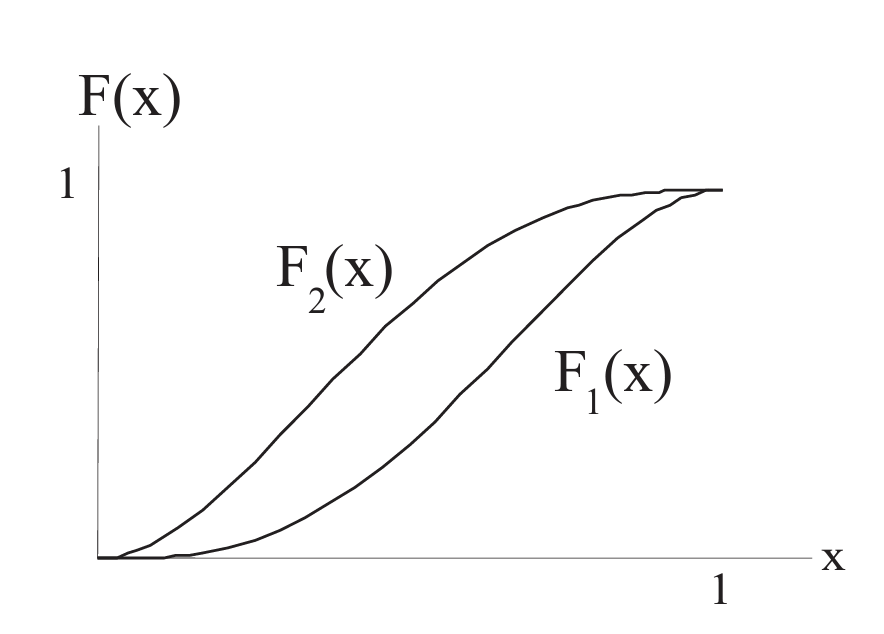
\includegraphics[scale=0.2]{FOSD_1.png}
    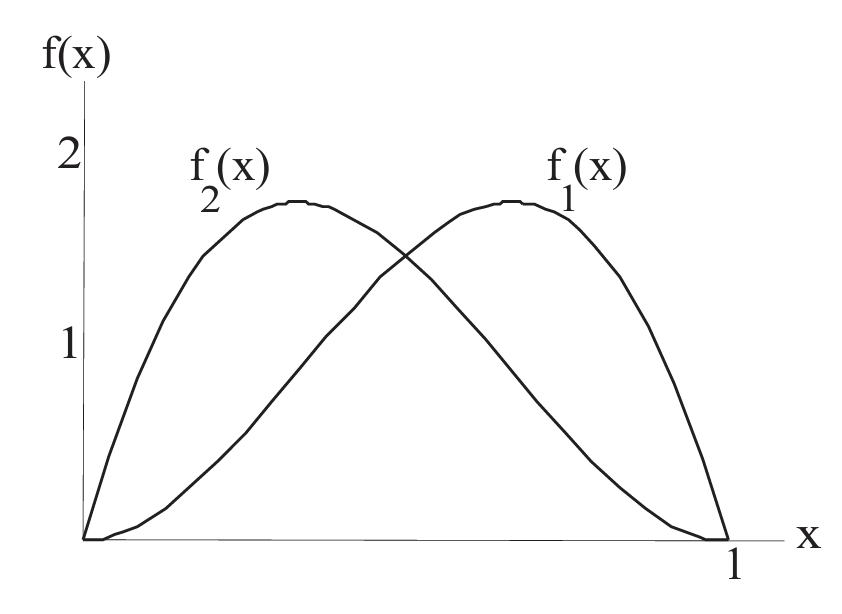
\includegraphics[scale=0.2]{FOSD_2.png}
    \caption{$F_1$ is FOSD over $F_2$: CDF and density comparison}
    \label{}
\end{figure}\end{center}

\section{Second-order Stochastic Dominance}
\subsection{Definition in terms of final goals}
\begin{definition}[Second-order Stochastic Dominance]
    \normalfont
    For any lotteries $F$ and $G$, $F$ \textbf{second-order stochastically dominates} $G$ if and only if the decision maker weakly prefers $F$ to $G$ under every \underline{weakly \textbf{increasing concave}} utility function $u$, i.e.,
    $$\int u (x) dF \geq \int u(x) dG$$
\end{definition}
\begin{center}\begin{figure}[htbp]
    \centering
    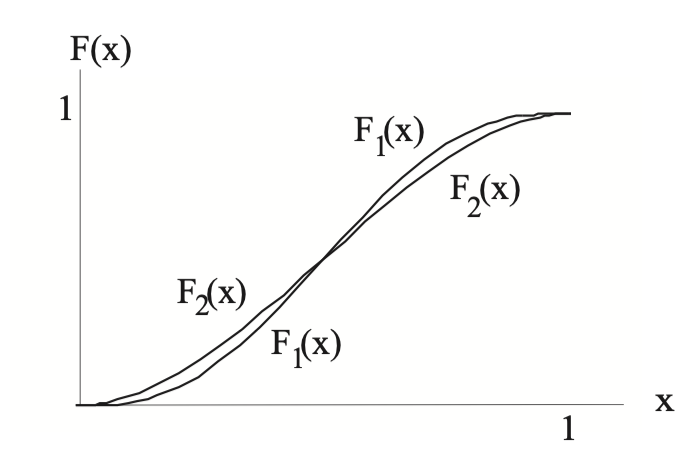
\includegraphics[scale=0.25]{SOSD_1.png}
    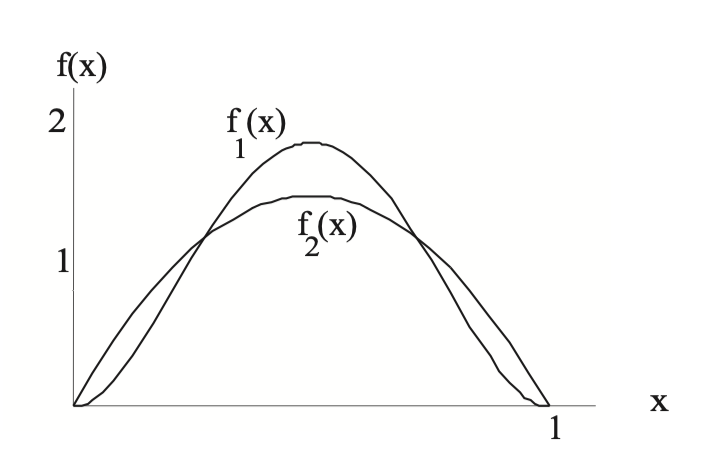
\includegraphics[scale=0.25]{SOSD_2.png}
    \caption{$F_1$ is SOSD over $F_2$: CDF and density comparison}
    \label{}
\end{figure}\end{center}

\subsection{Mean-Preserving Spread/Contraction}
\begin{definition}[Mean-Preserving Spread]
    \normalfont
    Let $x_F$ and $x_G$ be the random variables associated with lotteries $F$ and $G$. Then $G$ is a \textbf{mean-preserving spread} of $F$ if and only if $$x_G \stackrel{d}{=} x_F+\varepsilon$$
    for some random variable $\varepsilon$ such that $\mathbb{E}(\varepsilon\mid x_F)=0\ \forall x_F$.
\end{definition}
The "$\stackrel{d}{=}$" means "is equal in distribution to" (that is, "has the same distribution as").

\begin{note}
    Given $G$ is a \textbf{mean-preserving spread} of $F$, $G$ has larger variance than $F$.
\end{note}

\begin{example}
    $F(198)=\frac{1}{2}, F(202)=\frac{1}{2}$ and $G(100)=\frac{1}{100}$, $G(200)=\frac{98}{100}$, $G(300)=\frac{1}{100}$. Then $$x_G \stackrel{d}{=} x_F+\varepsilon$$
    where the distribution of $\varepsilon$ can be solved by $$\left\{\begin{matrix}
        G(300)=F(198)P(\varepsilon=102|x_F=198)+F(202)P(\varepsilon=98|x_F=202)\\
        G(200)=F(198)P(\varepsilon=2|x_F=198)+F(202)P(\varepsilon=-2|x_F=202)\\
        G(100)=F(198)P(\varepsilon=-98|x_F=198)+F(202)P(\varepsilon=-102|x_F=202)
    \end{matrix}\right.$$
\end{example}


\subsection{For Same Mean Distributions, Second-order Stochastic Dominance is equivalent to Mean-Preserving Spread}
\begin{theorem}[Second-order Stochastic Dominance Equivalence]\label{SOSD_equiv}
    Given $\int x dF=\int x dG$ (same mean). The following are equivalent.
    \begin{enumerate}
        \item $F$ second-order stochastically dominates $G$: $\int u (x) dF \geq \int u(x) dG$  for every weakly increasing concave utility function $u$.
        \item $F$ is a mean-preserving contraction of $G$ ($G$ is a mean-preserving spread of $F$).
        \item For every $t\geq 0$, $\int_a^t G(x)dx\geq \int_a^t F(x)dx$.
    \end{enumerate}
\end{theorem}
\begin{center}\begin{figure}[htbp]
    \centering
    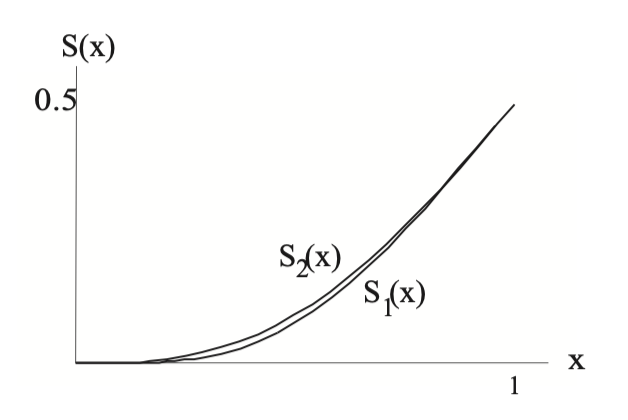
\includegraphics[scale=0.25]{SOSD_3.png}
    \caption{$F_1$ is SOSD over $F_2$, $S(t):\int_a^t F_2(x)dx\geq \int_a^t F_1(x)dx$}
    \label{}
\end{figure}\end{center}

\begin{corollary}[Euqivalent Definitions of MPC and MPS]
    \normalfont
    $F$ is a mean-preserving contraction of $G$ (or $G$ is a mean-preserving spread of $F$) \underline{if and only if}
    \begin{enumerate}[(1).]
        \item $\int x dF=\int x dG$
        \item $\int_a^t G(x)dx\geq \int_a^t F(x)dx, \forall t$
    \end{enumerate}
\end{corollary}

\begin{corollary}[$\textnormal{MPC}(f)$ and $\textnormal{MPS}(f)$ are convex and compact]
    $\textnormal{MPC}(f)$ and $\textnormal{MPS}(f)$ are \textbf{convex} and \textbf{compact}.
\end{corollary}




\chapter{Tools for Comparative Statics}
Consider the function $f:(0,2\pi) \times \mathbb{R} \rightarrow \mathbb{R}$ s.t. $$f(x,a)=\sin x+a$$
Let $X=(0,2\pi)$ and let $f_a(x) = f(x, a) = \sin x + a$ denote the perturbed function for fixed $a$.



\section{Regular and Critical Points and Values}
\subsection{Rank of Derivatives $\textnormal{Rank} df_x=\textnormal{Rank} Df(x)$}
Suppose $X \subseteq \mathbb{R}^n$ is open. Suppose $f : X \rightarrow \mathbb{R}^m$ is differentiable at $x \in X$, and let $W = \{e_1, . . . , e_n\}$ denote the standard basis of $\mathbb{R}^n$. Then $df_x \in L(\mathbb{R}^n, \mathbb{R}^m)$, and
\begin{equation}
    \begin{aligned}
        \textnormal{Rank} df_x &= \dim \textnormal{Im}(df_x)\\
        &= \dim \textnormal{span}\{df_x(e_1), . . . , df_x(e_n)\}\\
        &= \dim \textnormal{span}\{Df(x)e_1, . . . , Df(x)e_n\}\\
        &= \dim \textnormal{span}\{\textnormal{column 1 of }Df(x), . . . , \textnormal{column n of }Df(x)\}\\
        &=\textnormal{Rank} Df(x)
    \end{aligned}
    \nonumber
\end{equation}
Thus,
$$\textnormal{Rank} df_x\leq\min\{m,n\}$$
$df_x$ has \textbf{full rank} if $\textnormal{Rank} df_x=\min\{m,n\}$, that is, is $df_x$ has the maximum possible rank.

\subsection{Regular and Critical Points and Values}
\begin{definition}[Regular and Critical Points and Values]
    \normalfont
    Suppose $X \subseteq \mathbb{R}^n$ is open. Suppose $f : X \rightarrow \mathbb{R}^m$ is differentiable at $x \in X$.
    \begin{enumerate}
        \item $x$ is a \textbf{regular point} of $f$ if $\textnormal{Rank} df_x=\min\{m,n\}$.
        \item $x$ is a \textbf{critical point} of $f$ if $\textnormal{Rank} df_x<\min\{m,n\}$.
        \item $y$ is a \textbf{critical value} of $f$ if  there exists $x \in f^{-1}(y)$ such that $x$ is a critical point of $f$.
        \item $y$ is a \textbf{regular value} of $f$ if $y$ is not a critical value of $f$.
    \end{enumerate}
\end{definition}
\begin{note}
    Notice that if $y \notin f(X)$, so $f^{-1}(y) = \emptyset$, then $y$ is automatically a regular value of $f$.
\end{note}

\begin{example}
    Suppose $f(x,y)=(\sin x,\cos y)$, $Df(x,y)=\begin{bmatrix}
        \cos x&	0\\
        0&	-\sin y
    \end{bmatrix}$. Critical point: $\{(\frac{k\pi}{2}, \mathbb{R}): k\in 2\mathbb{Z}+1\}\cup\{(\mathbb{R},k\pi): k\in \mathbb{Z}\}$; Critical values: $\{(x,y): x=1\textnormal{ or }x=-1 \textnormal{ or }y=1\textnormal{ or }y=-1\}$
\end{example}


\section{Inverse and Implicit Function Theorem}
\subsection{Inverse Function Theorem}
Using Taylor's theorem to approximate
\begin{equation}
    \begin{aligned}
        f(x)=f(x_0)+Df(x_0)(x-x_0)+o(x-x_0)
    \end{aligned}
    \nonumber
\end{equation}
The requirement of "regular point" is necessary for the $Df(x_0)$ being invertible.
\begin{theorem}[Inverse Function Theorem]
    Suppose $X \subseteq \mathbb{R}^n$ is open. Suppose $f : X \rightarrow \mathbb{R}^n$ is $C^1$ on $X$, and $x_0\in X$. If $\det Df(x_0)\neq 0$ (i.e., $x_0$ is a regular point of $f$), then there are open neighborhoods $U$ of $x_0$ and $V$ of $f(x_0)$ s.t.
    \begin{equation}
        \begin{aligned}
            &f:U \rightarrow V \textnormal{ is bijective (on-to-on and onto)}\\
            &\exists\ f^{-1}:V \rightarrow U \textnormal{ is }C^1\\
            &Df^{-1}(f(x_0))=[Df(x_0)]^{-1}\\
            &\textnormal{(In $\mathbb{R}$, $(f^{-1})'(f(x_0))=(f'(x_0))^{-1}$)}
        \end{aligned}
        \nonumber
    \end{equation}
    If in addition $f \in C^k$, then $f^{-1} \in C^k$.
\end{theorem}

\subsection{Implicit Function Theorem}
Using Taylor's theorem to approximate
\begin{equation}
    \begin{aligned}
        f(x,a)=f(x_0,a_0)+Df(x_0,a_0)(x-x_0)+Df(x_0,a_0)(a-a_0)+\textnormal{remainder}
    \end{aligned}
    \nonumber
\end{equation}
The requirement of "regular point" is necessary for the $Df(x_0,a_0)$ being invertible.

We want to know how the function $x^*(a)$ changes with keeping $f(x^*,a)=0$.
\begin{theorem}[Implicit Function Theorem]
    Suppose $X \subseteq \mathbb{R}^n$ and $A \subseteq \mathbb{R}^p$ are open and $f : X \times A \rightarrow \mathbb{R}^n$ is $C^1$. Suppose $f(x_0, a_0) = 0$ and $\det(D_x f(x_0, a_0)) \neq 0$, i.e. $x_0$ is a regular point of $f(\cdot, a_0)$. Then there are open neighborhoods $U$ of $x_0$ ($U \subseteq X$) and $W$ of $a_0$ such that
    $$\forall a\in W,\ \exists ! x\in U \textnormal{ s.t. }f(x,a)=0$$
    For each $a \in W$ let $g(a)$ be that unique $x$. Then $g : W \rightarrow U$ is $C^1$ and $$Dg(a_0)=-[D_x f(x_0, a_0)]^{-1}[D_a f(x_0, a_0)]$$
    If in addition $f \in C^k$, then $g \in C^k$.
\end{theorem}
\subsection{Prove Implicit Function Theorem Given Inverse Function Theorem}
\begin{proof}
    \begin{enumerate}
        \item Firstly, we prove "$g$ is differentiable":
        The "change of $a$" incurs the value change:
        \begin{equation}
            \begin{aligned}
                f(x_0,a_0+h)&=f(x_0,a_0)+D_af(x_0,a_0)h+o(h)\\
                &=D_af(x_0,a_0)h+o(h)\\
            \end{aligned}
            \nonumber
        \end{equation}
        Find a $\Delta x$ such that the new $x$ can let the value go back to $0$, i.e., $f(x_0+\Delta x,a_0+h)=0$. That is,
        \begin{equation}
            \begin{aligned}
                g(a_0+h)=x_0+\Delta x
            \end{aligned}
            \nonumber
        \end{equation}
        To prove "$g$ is differentiable", we want to prove "$\exists T\in L(A,X)$ s.t. $\Delta x=T(h)+o(h)$"
        \begin{equation}
            \begin{aligned}
                0&=f(x_0+\Delta x,a_0+h)\\
                &=f(x_0,a_0)+D_xf(x_0,a_0+h)\Delta x+ D_a f(x_0,a_0)h+o(\Delta x)+o(h)\\
                &=D_xf(x_0,a_0+h)\Delta x+ D_a f(x_0,a_0)h+o(\Delta x)+o(h)\\
                D_x f(x_0,a_0+h)\Delta x&=-D_a f(x_0,a_0)h+o(\Delta x)+o(h)
            \end{aligned}
            \nonumber
        \end{equation}
        Because $f$ is $C^1$ and the determinant is a continuous function of the entries of the matrix, $\det D_xf(x_0, a_0 + h) \neq 0$ for $h$ sufficiently small, so
        \begin{equation}
            \begin{aligned}
                \Delta x&= -[D_x f(x_0,a_0+h)]^{-1}D_a f(x_0,a_0)h+o(\Delta x)+o(h)\\
                \textnormal{Since $f\in C^1$, }\Delta x&= -[D_x f(x_0,a_0)+o(1)]^{-1}D_a f(x_0,a_0)h+o(\Delta x)+o(h)\\
                \textnormal{Since $f\in C^1$, }\Delta x&= -[D_x f(x_0,a_0)]^{-1}D_a f(x_0,a_0)h+o(\Delta x)+o(h)
            \end{aligned}
            \nonumber
        \end{equation}
        Hence, "$g$ is differentiable" is proved and the derivative of $g$ is $Dg(a_0)=-[D_x f(x_0,a_0)]^{-1}[D_a f(x_0,a_0)]$.
        \item Secondly, given the "$g$ is differentiable", we can also compute the derivative by
        \begin{equation}
            \begin{aligned}
                Df(g(a),a)(a_0)&=0\\
                D_xf(x_0,a_0)Dg(a_0)+D_af(x_0,a_0)&=0\\
                Dg(a_0)&=-[D_x f(x_0,a_0)]^{-1}D_a f(x_0,a_0)
            \end{aligned}
            \nonumber
        \end{equation}
    \end{enumerate}
\end{proof}







\begin{example}
    $f: \mathbb{R}^3 \rightarrow \mathbb{R}^2$, $f((3,-1,2))=(0,0)$, $Df(3,-1,2)=\begin{bmatrix}
        1&2&1\\
        1&-1&1
    \end{bmatrix}$. Then,
    let $(x_0,a_0)=(3,-1,2)$, where $x_0=3$ and $a_0=(-1,2)$. Or, we can let $(x_0,a_0)=(3,-1,2)$, where $x_0=(3,-1)$ and $a_0=2$.
\end{example}

\subsection{Prove Inverse Function Theorem Given Implicit Function Theorem}
\begin{proof}[Prove Inverse Function Theorem Given Implicit Function Theorem]
    Define $F:X\times \mathbb{R}^n$ s.t. $F(x,y)=y-f(x)$. Let $y_0=f(x_0)$.
    \begin{equation}
        \begin{aligned}
            D_x F(x,y)=-Df(x),\ D_y F(x,y)=I_{n\times n}
        \end{aligned}
        \nonumber
    \end{equation}
    According to the implicit function theorem, there are open sets $U \subseteq X$ and $V \subseteq \mathbb{R}^n$ such that $x_0 \in U$, $y_0 \in V$ and a function $g : V \rightarrow U$ differentiable at $y_0$ such that $F(g(y), y) = 0$ for all $y \in V$. So, $0=F(g(y),y)=y-f(g(y))$, we have $f(g(y))=y$, that is $g=f^{-1}$.
    $f: U \rightarrow V$ is bijective because it has inverse $g : V \rightarrow U$.

    By the implicit function theorem, $g(y)$ is differentiable and
    \begin{equation}
        \begin{aligned}
            Df^{-1}(y_0)=Dg(y_0)=-[D_x F(x_0,y_0)]^{-1}[D_y F(x_0,y_0)]=[Df(x_0)]^{-1}
        \end{aligned}
        \nonumber
    \end{equation}
    where $y_0=f(x_0)$.
    
    By the implicit function theorem, the $g=f^{-1}$ is $C^k$ if $f$ is $C^k$.

    All in all, the inverse function theorem is proved.
\end{proof}

\subsection{Example: Using Implicit Function Theorem}
%Consider $u_1(a)=ba-ka^2$, where $a^*=\frac{b}{2k}$.

%More general, $U(a)=b(a)-c(a)$. $a^*$ solve $b'(a)-c'(a)=0$.

$x^2+y^2=c$. Define $g(x,y)=x^2+y^2-c$. The optimal solution of $y$ given $x$ is represented by $y^*(x)$. By the implicit function theorem,
\begin{equation}
    \begin{aligned}
        \frac{\partial y^*}{\partial x}=-\frac{\frac{\partial g}{\partial x}\big|_{x,y^*}}{\frac{\partial g}{\partial y}\big|_{x,y^*}}
    \end{aligned}
    \nonumber
\end{equation}


\begin{example}
    Let us consider a firm that produces a good $y$; it uses two inputs $x_1$ and $x_2$. The firm sells the output and acquires the inputs in competitive markets: The market price of $y$ is $p$, and the cost of each unit of $x_1$ and $x_2$ are $w_1$ and $w_2$ respectively. Its technology is given by $f : \mathbb{R}^2_+ \rightarrow \mathbb{R}_+$, where $f (x_1, x_2) = x_1^ax_2^b$, $a + b < 1$. Its profits take the form
    \begin{equation}
        \begin{aligned}
            \pi(x_1,x_2; p, w_1,w_2)=p x_1^ax_2^b-w_1x_1-w_2x_2
        \end{aligned}
        \nonumber
    \end{equation}
    The firm selects $x_1$ and $x_2$ in order to maximize profits. \textbf{We aim to know how its choice of $x_1$ and $x_2$ is affected by a change in $w_1$}.

    Assuming an interior solution, the first-order conditions of this optimization problem are
    \begin{equation}
        \begin{aligned}
            \frac{\partial \pi}{\partial x_1}(x_1^*,x_2^*;p,w_1,w_2)=pa(x_1^*)^{a-1}(x_2^*)^b-w_1=0\\
            \frac{\partial \pi}{\partial x_2}(x_1^*,x_2^*;p,w_1,w_2)=pb(x_1^*)^{a}(x_2^*)^{b-1}-w_2=0
        \end{aligned}
        \nonumber
    \end{equation}
    for some $(x_1, x_2) = (x_1^*,x_2^*)$.

    Let us define
    \begin{equation}
        \begin{aligned}
            F(x_1^*,x_2^*;p,w_1,w_2)=
            \begin{bmatrix}
                pa(x_1^*)^{a-1}(x_2^*)^b-w_1\\
                pb(x_1^*)^{a}(x_2^*)^{b-1}-w_1
            \end{bmatrix}
        \end{aligned}
        \nonumber
    \end{equation}
    Jacobian matrices are
    \begin{equation}
        \begin{aligned}
            D_{(x_1,x_2)}F(x_1^*,x_2^*;p,w_1,w_2)=\begin{bmatrix}
                pa(a-1)(x_1^*)^{a-2}(x_2^*)^b&pab(x_1^*)^{a-1}(x_2^*)^{b-1}\\
                pab(x_1^*)^{a-1}(x_2^*)^{b-1}&pb(b-1)(x_1^*)^{a}(x_2^*)^{b-2}
            \end{bmatrix}
        \end{aligned}
        \nonumber
    \end{equation}
    \begin{equation}
        \begin{aligned}
            D_{w_1}F(x_1^*,x_2^*;p,w_1,w_2)
            &=
            \begin{bmatrix}
                -1\\
                0
            \end{bmatrix}
        \end{aligned}
        \nonumber
    \end{equation}
    By the implicit function theorem, we can get
    \begin{equation}
        \begin{aligned}
            \begin{bmatrix}
                \frac{\partial x_1^*}{\partial w_1}\\
                \frac{\partial x_2^*}{\partial w_1}
            \end{bmatrix}&=-[D_{(x_1,x_2)}F(x_1^*,x_2^*;p,w_1,w_2)]^{-1}[D_{w_1}F(x_1^*,x_2^*;p,w_1,w_2)]\\
            &=[D_{(x_1,x_2)}F(x_1^*,x_2^*;p,w_1,w_2)]^{-1}\begin{bmatrix}
                1\\
                0
            \end{bmatrix}
        \end{aligned}
        \nonumber
    \end{equation}
\end{example}

\subsection{Corollary: $a \rightarrow \{x\in X: f(x,a)=0\}$ is lhc}
\begin{corollary}
    Suppose $X \subseteq \mathbb{R}^n$ and $A \subseteq \mathbb{R}^p$ are open and $f : X \times A \rightarrow \mathbb{R}^n$ is $C^1$. If $0$ is a regular value of $f(\cdot, a_0)$, then the correspondence $$a \rightarrow \{x\in X: f(x,a)=0\}$$
    is \textbf{lower hemicontinuous} at $a_0$.
\end{corollary}

\section{Transversality and Genericity}
\subsection{Lebesgue Measure Zero}
\begin{definition}[Lebesgue Measure Zero]
    \normalfont
    Suppose $A \subseteq \mathbb{R}^n$. $A$ has \textbf{Lebesgue measure zero} if for every $\varepsilon > 0$ there is a countable collection of rectangles $I_1, I_2, . . .$ such that
    \begin{equation}
        \begin{aligned}
            \sum_{k=1}^\infty\textnormal{Vol}(I_k)<\varepsilon \textnormal{ and }A\subseteq \cup_{k=1}^\infty I_k
        \end{aligned}
        \nonumber
    \end{equation}
    Here by a rectangle we mean $I_k = \times^n_{j=1}(a^k_j , b^k_j)=\{x\in \mathbb{R}^n: x_j\in (a^k_j , b^k_j), \forall j\}$ for some $a^k_j < b^k_j \in \mathbb{R}$, and
    \begin{equation}
        \begin{aligned}
            \textnormal{Vol}(I_k)=\prod_{j=1}^n|b^k_j-a^k_j|
        \end{aligned}
        \nonumber
    \end{equation}
\end{definition}

\begin{example}
    \begin{enumerate}
        \item “Lower-dimensional” sets have Lebesgue measure zero. For example, $A=\{x\in\mathbb{R}^2:x_2=0\}$
        \item Any \textbf{finite} set has Lebesgue measure zero in $\mathbb{R}^n$.
        \item \textbf{Finite Union} of sets that have Lebesgue measure zero has Lebesgue measure zero: If $A_n$ has Lebesgue measure zero $\forall n$ then $\cup_{n\in N}A_n$ has Lebesgue measure zero.
        \item Every \textbf{countable} set (e.g. $\mathbb{Q}$) has Lebesgue measure zero.
        \item No open set in $\mathbb{R}^n$ has Lebesgue measure zero.
    \end{enumerate}
\end{example}


\subsection{Sard's Theorem}
\begin{theorem}[Sard's Theorem]
    Let $X \subseteq \mathbb{R}^n$ be open, and $f : X \rightarrow \mathbb{R}^m$ be $C^r$ with $r \geq 1 + max\{0, n - m\}$. Then the set of all critical values of $f$ has Lebesgue measure zero.
\end{theorem}

\subsection{Transversality Theorem}
\begin{theorem}[Transversality Theorem]
    Let $X \subseteq \mathbb{R}^n$ and $A \subseteq \mathbb{R}^p$ be open, and $f : X \times A \rightarrow \mathbb{R}^m$ be $C^r$ with $r \geq 1 + max\{0, n - m\}$. Suppose that $0$ is a regular value of $f$ (that is all $(x,a)$ such that $f(x,a)=0$ are regular points). Then,
    \begin{enumerate}
        \item $\exists A_0 \subseteq A$ such that $A \backslash A_0$ has Lebesgue measure zero.
        \item $\forall a \in A_0$, $0$ is a regular value of $f_a = f(\cdot, a)$.
    \end{enumerate}
\end{theorem}
\begin{example}
    $f: \mathbb{R}^4 \rightarrow \mathbb{R}^3$ s.t. $f(x,y,z,w)=(g(x)+y,z^3+1,w+x+y^2)$
\end{example}


\chapter{Fixed Point Theorem}

\section{Contraction Mapping Theorem \small{(@ Lec 05 of ECON 204)}}
\subsection{Contraction: Lipschitz continuous with constant $<1$}
\begin{definition}
    \normalfont
    Let $(X, d)$ be a \underline{nonempty complete} metric space. An operator is a function $T : X \rightarrow X$. An operator $T$ is a \textbf{contraction of modulus $\beta$} if $\beta < 1$ and $$d(T(x), T(y)) \leq \beta d(x, y), \forall x,y\in X$$
\end{definition}
A contraction shrinks distances by a \textit{uniform} factor $\beta < 1$.

\subsection{Theorem: Contraction $\Rightarrow$ Uniformly Continuous}
\begin{theorem}[Contraction $\Rightarrow$ Uniformly Continuous]
    Every contraction is uniformly continuous.
\end{theorem}
\begin{proof}
    Let $\delta=\frac{\varepsilon}{\beta}$.
\end{proof}

\subsection{Blackwell's Sufficient Conditions for Contraction}
Let $X$ be a set, and let $B(X)$ be the set of all bounded functions from $X$ to $\mathbb{R}$. Then $(B(X), \|\cdot\|_\infty)$ is a normed vector space.

(Notice that below we use shorthand notation that identifies a constant function with its constant value in $\mathbb{R}$, that is, we write interchangeably $a \in \mathbb{R}$ and $a : X \rightarrow \mathbb{R}$ to denote the function such that $a(x) = a, \forall x \in X$.)

\begin{theorem}[Blackwell's Sufficient Conditions]
    Consider $B(X)$ with the sup norm $\|\cdot\|_\infty$. Let $T : B(X) \rightarrow B(X)$ be an operator satisfying
    \begin{enumerate}
        \item (monotonicity) $f(x) \leq g(x), \forall x\in X \Rightarrow (T f)(x) \leq (T g)(x), \forall x \in X$
        \item (discounting) $\exists \beta \in (0, 1)$ such that for every $a \geq 0$ and $x \in X$, $$(T (f + a)) (x) \leq (T f)(x) + \beta a$$
    \end{enumerate}
    Then $T$ is a contraction with modulus $\beta$.
\end{theorem}
\begin{proof}
    Fix $f, g \in B(X)$. By the definition of the sup norm,
    $$
    f(x) \leq g(x)+\|f-g\|_{\infty} \forall x \in X
    $$
    Then
    $$
    (T f)(x) \leq\left(T\left(g+\|f-g\|_{\infty}\right)\right)(x) \leq(T g)(x)+\beta\|f-g\|_{\infty} \quad \forall x \in X
    $$
    where the first inequality above follows from monotonicity, and the second from discounting. Thus
    $$
    (T f)(x)-(T g)(x) \leq \beta\|f-g\|_{\infty} \quad \forall x \in X
    $$
    Reversing the roles of $f$ and $g$ above gives
    $$
    (T g)(x)-(T f)(x) \leq \beta\|f-g\|_{\infty} \quad \forall x \in X
    $$
    Thus
    $$
    \|T(f)-T(g)\|_{\infty} \leq \beta\|f-g\|_{\infty}
    $$
    Thus $T$ is a contraction with modulus $\beta$
\end{proof}


\section{Fixed Point Theorem \small{(@ Lec 05 of ECON 204)}}
\subsection{Fixed Point}
\begin{definition}[Fixed Point]
    \normalfont
    A \textbf{fixed point} of an operator $T$ is element $x^*\in X$ such that $T(x^*)=x^*$.
\end{definition}

\begin{definition}[Fixed Point of Function]
    \normalfont
    Let $X$ be a nonempty set and $f : X \rightarrow X$. A point $x^* \in X$ is a \textbf{fixed point} of $f$ if $f(x^*) = x^*$.
\end{definition}

\begin{example}
    Let $X=\mathbb{R}$ and $f: \mathbb{R} \rightarrow \mathbb{R}$
    \begin{enumerate}
        \item $f(x)=2x$ has fixed point: $x=0$.
        \item $f(x)=x$ has fixed points: $x\in \mathbb{R}$.
        \item $f(x)=x+1$ doesn't have fixed points.
    \end{enumerate}
\end{example}

\subsection{$\bigstar$ Contraction Mapping Theorem: contraction $\Rightarrow$ exist unique fixed point}
\begin{theorem}[Contraction Mapping Theorem]
    Let $(X, d)$ be a nonempty complete metric space and $T : X \rightarrow X$ a contraction with modulus $\beta < 1$. Then
    \begin{enumerate}
        \item $T$ has a unique fixed point $x^*$.
        \item For every $x_0 \in X$, the sequence defined by
        \begin{equation}
            \begin{aligned}
                x_1&=T(x_0)\\
                x_2&=T(x_1)=T(T(x_0))=T^2(x_0)\\
                &\vdots\\
                x_{n+1}&=T(x_n)=T^{n+1}(x_0)
            \end{aligned}
            \nonumber
        \end{equation}
        converges to $x^*$.
    \end{enumerate}
\end{theorem}
Note that the theorem asserts both the \textbf{existence} and \textbf{uniqueness} of the fixed point, as well as giving an \textbf{algorithm} to find the fixed point of a contraction.
\begin{proof}
    Define the sequence $\{x_n\}$ as above. Then,
    \begin{equation}
        \begin{aligned}
            d(x_{n+1},x_n)&=d(T(x_n),T(x_{n-1}))\\
            &\leq \beta d(x_n,x_{n-1})\\
            &\leq \beta^n d(x_1,x_0)
        \end{aligned}
        \nonumber
    \end{equation}
    Then for any $n>m$,
    \begin{equation}
        \begin{aligned}
            d(x_n,x_m)&\leq d(x_1, x_0) \sum_{i=m}^{n-1}\beta^i\\
            &<d(x_1, x_0) \sum_{i=m}^{\infty}\beta^i\\
            &=\frac{\beta^m}{1-\beta}d(x_1, x_0) \rightarrow 0 \textnormal{ as }m \rightarrow \infty
        \end{aligned}
        \nonumber
    \end{equation}
    Fixed $\varepsilon>0$, we can choose $N(\varepsilon)$ such that $\forall n,m>N(\varepsilon)$, $$d(x_n,x_m)<\frac{\beta^m}{1-\beta}d(x_1, x_0) <\varepsilon$$
    Therefore, $\{x_n\}$ is Cauchy. Since $(X, d)$ is complete, $x_n \rightarrow x^*$ for some $x^*\in X$.

    Next we show that $x^*$ is a fixed point of $T$.
    $$
    \begin{aligned}
    T\left(x^*\right) & =T\left(\lim _{n \rightarrow \infty} x_n\right) \\
    & =\lim _{n \rightarrow \infty} T\left(x_n\right) \text { since } T \text { is continuous } \\
    & =\lim _{n \rightarrow \infty} x_{n+1} \\
    & =x^*
    \end{aligned}
    $$
    so $x^*$ is a fixed point of $T$.
    
    Finally, we show that there is at most one fixed point. Suppose $x^*$ and $y^*$ are both fixed points of $T$, so $T\left(x^*\right)=x^*$ and $T\left(y^*\right)=y^*$. Then
    $$
    \begin{aligned}
    d\left(x^*, y^*\right) & =d\left(T\left(x^*\right), T\left(y^*\right)\right) \\
    & \leq \beta d\left(x^*, y^*\right) \\
    \Rightarrow(1-\beta) d\left(x^*, y^*\right) & \leq 0 \\
    \Rightarrow d\left(x^*, y^*\right) & \leq 0
    \end{aligned}
    $$
    So $d\left(x^*, y^*\right)=0$, which implies $x^*=y^*$.
\end{proof}



\subsection{Conditions for Fixed Point's Continuous Dependence on Parameters}
\begin{theorem}[Continuous Dependence on Parameters]
    Let $(X, d)$ and $(\Omega, \rho)$ be two metric spaces and $T : X \times \Omega \rightarrow X$. For each parameter $\omega \in \Omega$ let $T_\omega : X \rightarrow X$ be defined by $T_\omega(x)=T(x,\omega)$.

    Suppose (1). $(X, d)$ is complete, (2). $T$ is continuous in $\omega$ (that is $T(x, \cdot) : \Omega \rightarrow X$ is continuous for each $x \in X$), and (3). $\exists \beta < 1$ such that $T_\omega$ is a contraction of modulus $\beta$ $\forall \omega \in \Omega$.
    
    Then the fixed point function (about parameter $\omega$) $x^*: \Omega \rightarrow X$ defined by $x^*(\omega)=T_\omega(x^*(\omega))$ is continuous.
\end{theorem}

\section{Brouwer's Fixed Point Theorem \small{(@ Lec 13 of ECON 204)}}
\subsection{Simple One: One-dimension}
\begin{theorem}
    Let $X = [a, b]$ for $a, b \in \mathbb{R}$ with $a < b$ and let $f : X \rightarrow X$ be continuous. Then $f$ has a fixed point.
\end{theorem}
\begin{proof}
    Easily proved by Intermediate Value Theorem.
\end{proof}

\subsection{$\bigstar$ Brouwer's Fixed Point Theorem: continuous function has fixed point over compact, convex set}
\begin{theorem}[Brouwer's Fixed Point Theorem]
    Let $X \subseteq \mathbb{R}^n$ be nonempty, \textbf{compact}, and \textbf{convex}, and let $f : X \rightarrow X$ be continuous. Then $f$ has a fixed point.
\end{theorem}
\begin{proof}
    \normalfont
    Consider the case when the set $X$ is the unit ball in $\mathbb{R}^n$.

    Using a fact that "Let $B$ be the unit ball in $\mathbb{R}^n$. Then there is no continuous function $h : B \rightarrow \partial B$ such that $h(x_0) = x_0$ for every $x_0 \in \partial B$", which is intuitive but hard to prove. (See \textit{J. Franklin, Methods of Mathematical Economics}, for an elementary (but long) proof.)

    Then prove by contradiction: suppose $f$ has no fixed points in $B$. That is, $\forall x\in B$, $x\neq f(x)$. Since x and its image $f(x)$ are distinct points in $B$ for every $x$, we can carry out the following construction. For each $x \in B$, construct the line segment originating at $f(x)$ and going through $x$. Let $g(x)$ denote the intersection of this line segment with $\partial B$. This construction gives a continuous function $g : B \rightarrow \partial B$. Furthermore, notice that if $x_0 \in \partial B$, then $x_0 = g(x_0)$. Then, $g$ gives $g(x)=x,\forall x\in \partial B$. Since there are no such functions by the fact above, we have a contradiction.
\end{proof}




\chapter{Correspondence: $\Psi : X \rightarrow 2^Y$ \small{(@ Lec 07 of ECON 204)}}
\begin{definition}[Correspondence]
    \normalfont
    A \textbf{correspondence} $\Psi : X \rightarrow 2^Y$ from $X$ to $Y$ is a function from $X$ to $2^Y$, that is, $\Psi(x) \subseteq Y$ for every $x \in X$. ($2^Y$ is the set of all subsets of $Y$)
\end{definition}
\begin{example}
Let $u : \mathbb{R}_+^n \rightarrow \mathbb{R}$ be a continuous utility function, $y > 0$ and $p \in \mathbb{R}_{++}^n$, that is, $p_i > 0$ for each $i$. Define $\Psi : \mathbb{R}_{++}^n \times \mathbb{R}_{++} \rightarrow 2^{\mathbb{R}_{+}^n}$ by
\begin{equation}
    \begin{aligned}
        \Psi(p,y)=&\argmax u(x)\\
        \textnormal{s.t. }&x\geq 0\\
        &p\cdot x\leq y
    \end{aligned}
    \nonumber
\end{equation}
$\Psi$ is the demand correspondence associated with the utility function $u$; typically $\Psi(p, y)$ is multi-valued.
\end{example}

\section{Continuity of Correspondences}
\subsection{Upper/Lower Hemicontinuous}
Let $X\subseteq \mathbb{E}^n$, $Y\subseteq \mathbb{E}^m$, and $\Psi: X \rightarrow 2^Y$.
\begin{definition}[Upper Hemicontinuous]
    \normalfont
    $\Psi$ is \textbf{upper hemicontinuous} (uhc) at $x_0 \in X$ if, for every \underline{open set} $V$ with $\Psi(x_0)\subseteq V$, there is an \underline{open set} $U$ with $x_0 \in U$ s.t.
    $$x\in U \Rightarrow \Psi(x)\subseteq V$$
\end{definition}
Upper hemicontinuity reflects the requirement that $\Psi$ doesn't “jump down/implode in the limit” at $x_0$. \textit{(A set to “jump down” at the limit $x_0$: It should mean the set suddenly gets smaller -- it “implodes in the limit” -- that is, there is a sequence $x_n \rightarrow x_0$ and points $y_n \in \Psi(x_n)$ that are far from every point of $\Psi(x_0)$ as $n \rightarrow \infty$.)}
\begin{definition}[Lower Hemicontinuous]
    \normalfont
    $\Psi$ is \textbf{lower hemicontinuous} (lhc) at $x_0 \in X$ if, for every \underline{open set} $V$ with $\Psi(x_0)\cap V \neq \emptyset$, there is an \underline{open set} $U$ with $x_0 \in U$ s.t.
    $$x\in U \Rightarrow \Psi(x)\cap V\neq \emptyset$$
\end{definition}
Lower hemicontinuity reflects the requirement that $\Psi$ doesn't “jump up/explode in the limit” at $x_0$. \textit{(A set to “jump up” at the limit $x_0$: It should mean that the set suddenly gets bigger -- it “explodes in the limit” -- that is, there is a sequence $x_n \rightarrow x_0$ and a point $y_0\in\Psi(x_0)$ that is far from every point of $\Psi(x_n)$ as $n \rightarrow \infty$.)}

\begin{definition}[Continuous Correspondence]
    \normalfont
    $\Psi$ is \textbf{continuous} at $x_0 \in X$ if it is both \textbf{uhc} and \textbf{lhc} at $x_0$.
\end{definition}

\begin{proposition}
    $\Psi$ is upper hemicontinuous (respectively lower hemicontinuous, continuous) if it is uhc (respectively lhc, continuous) at every $x \in X$.
\end{proposition}

\begin{center}\begin{figure}[htbp]
    \centering
    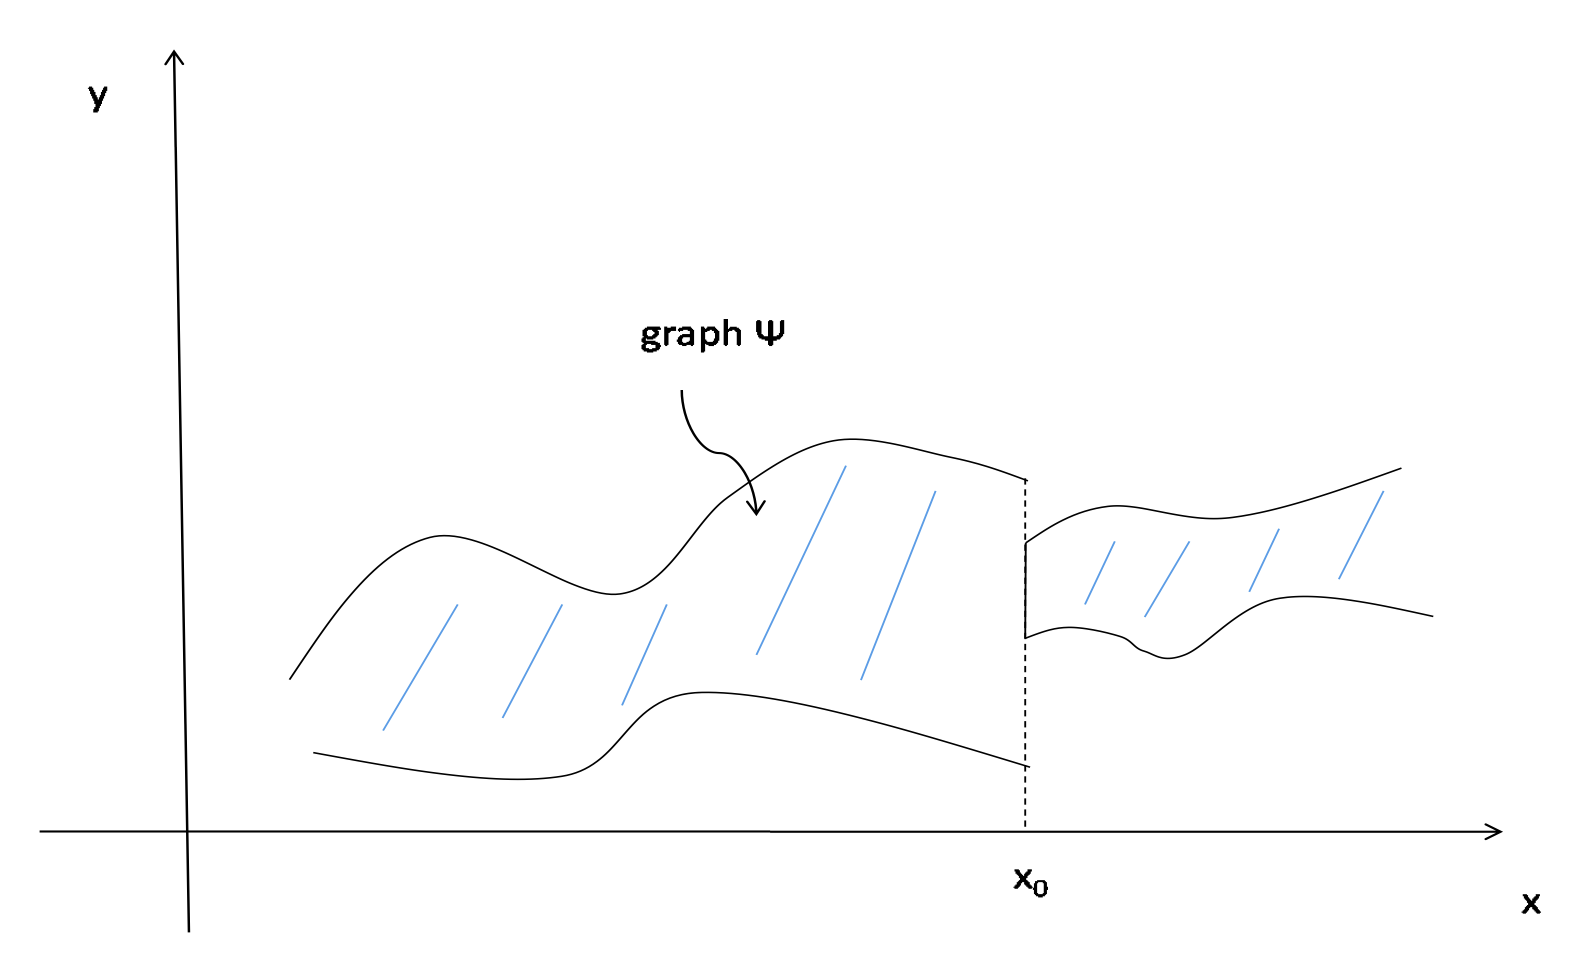
\includegraphics[scale=0.2]{uhc.png}
    \caption{The correspondence $\Psi$ “implodes in the limit” at $x_0$. $\Psi$ is not upper hemicontinuous at $x_0$.}
    \label{}
\end{figure}\end{center}

\begin{center}\begin{figure}[htbp]
    \centering
    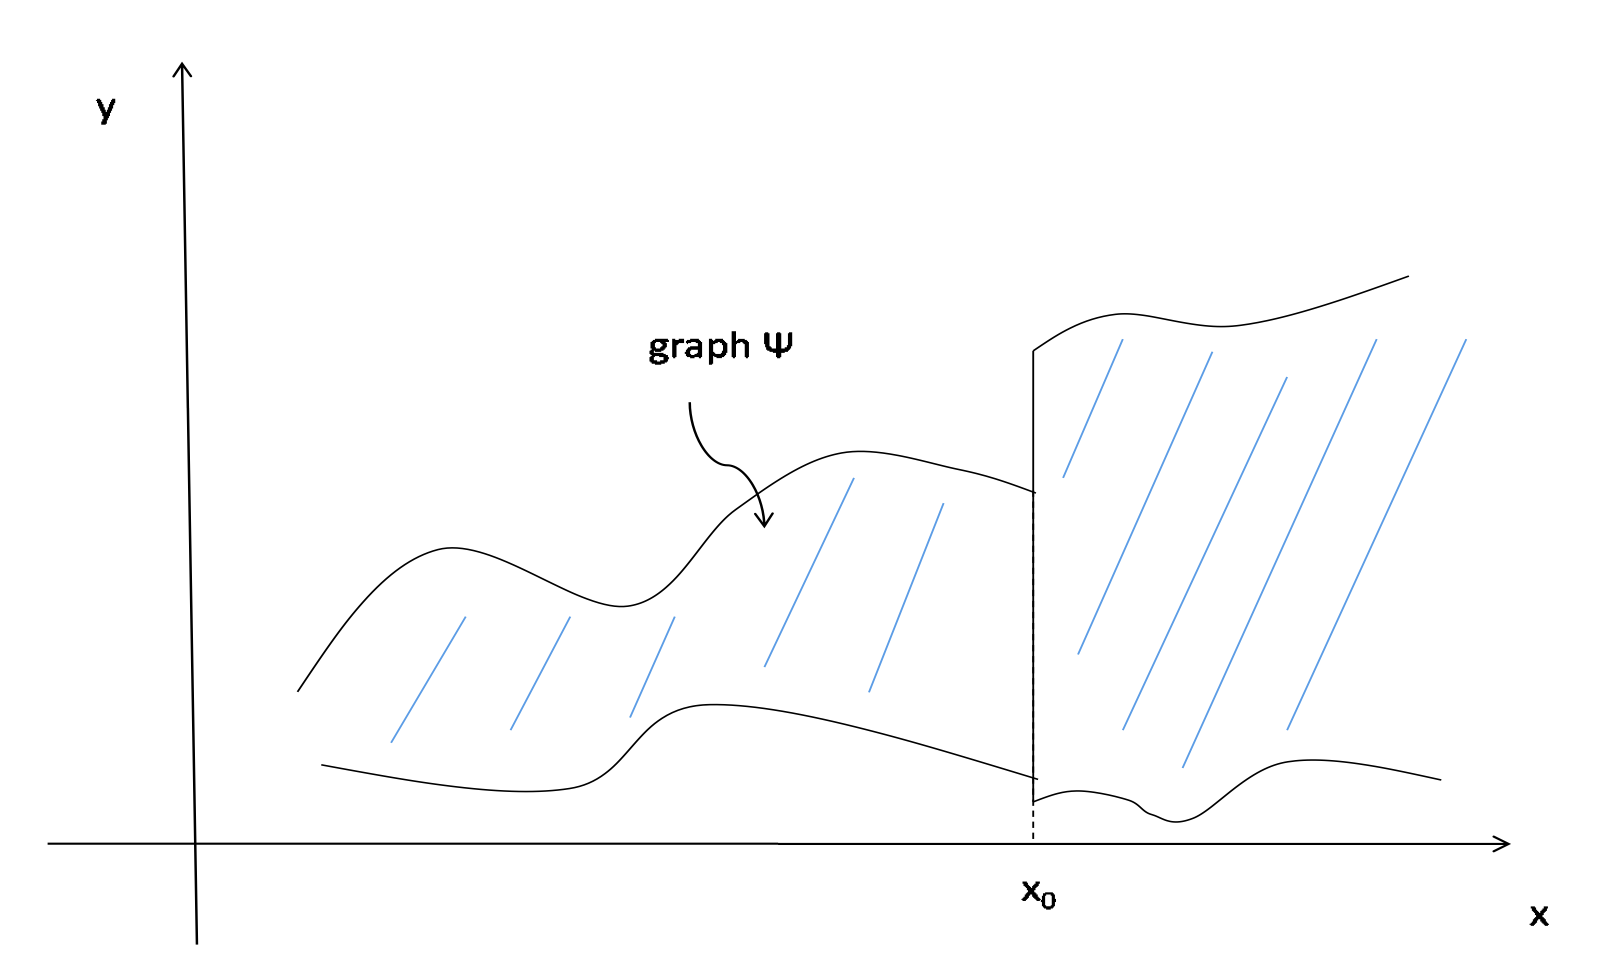
\includegraphics[scale=0.2]{lhc.png}
    \caption{The correspondence $\Psi$ “explodes in the limit” at $x_0$. $\Psi$ is not lower hemicontinuous at $x_0$.}
    \label{}
\end{figure}\end{center}

\subsection{Theorem: $\Psi(x)=\{f(x)\}$ is uhc $\Leftrightarrow$ $f$ is continuous}
\begin{theorem}[$\Psi(x)=\{f(x)\}$ is uhc $\Leftrightarrow$ $f$ is continuous]
    Let $X \subseteq \mathbb{E}^n$, $Y \subseteq \mathbb{E}^m$ and $f : X \rightarrow Y$. Let $\Psi : X \rightarrow  2^Y$ be defined by $\Psi(x) = \{f(x)\}$ for all $x \in X$. Then $\Psi$ is \textbf{uhc} \underline{if and only if} $f$ is \textbf{continuous}.
\end{theorem}


\subsection{Berge's Maximum Theorem: the set of maximizers is uhc with non-empty compact values}
\begin{theorem}[Berge's Maximum Theorem]\label{thm:Berge's Maximum Theorem}
    Let $X \subseteq \mathbb{R}^n$ and $Y \subseteq \mathbb{R}^m$. Consider the function $f : X \times Y \rightarrow \mathbb{R}$ and the correspondence $\Gamma : Y \rightarrow 2^X$. Define $v(y) = \max_{x\in\Gamma(y)} f(x, y)$ and the set of maximizers $$\Omega(y) = \argmax_{x\in\Gamma(y)} f(x, y)=\{x:f(x,y)=v(y)\}$$
    Suppose $f$ and $\Gamma$ are continuous, and that $\Gamma$ has non-empty compact values. Then, $v$ is continuous and $\Omega$ is uhc with non-empty compact values.
\end{theorem}




\section{Graph of Correspondence}
An alternative notion of continuity looks instead at properties of the graph of the correspondence.
\begin{definition}[Graph of Correspondence]
    \normalfont
    The \textbf{graph} of a correspondence $\Psi : X \rightarrow 2^Y$ is the set
    $$\textnormal{graph}\Psi=\{(x,y)\in X\times Y:y\in\Psi(x)\}$$
\end{definition}

\subsection{Closed Graph}
By the definition of continuous function $f:\mathbb{R}^n \rightarrow \mathbb{R}$,  each convergent sequence $\{(x_n, y_n)\}$ in graph $f$ converges to a point $(x, y)$ in graph $f$, that is, graph $f$ is closed.

\begin{definition}[Closed Graph]
    \normalfont
    Let $X\subseteq \mathbb{E}^n$, $Y\subseteq \mathbb{E}^m$. A correspondence $\Psi: X \rightarrow 2^Y$ has closed graph if its graph is a closed subset of $X \times Y$, that is, if for any sequences $\{x_n\} \subseteq X$ and $\{y_n\} \subseteq Y$ such that $x_n \rightarrow x \in X$, $y_n \rightarrow y \in Y$ and $y_n \in \Psi(x_n)$ for each $n$, then $y \in \Psi(x)$.
\end{definition}
\begin{example}
    Consider the correspondence $\Psi(x)=\left\{\begin{matrix}
        \{\frac{1}{x}\},&\textnormal{ if }x\in(0,1]\\
        \{0\},&\textnormal{ if }x=0
    \end{matrix}\right.$ ("implode in the limit")\\
    Let $V = (-0.1, 0.1)$. Then $\Psi(0) = \{0\} \subseteq V$, but no matter how close $x$ is to $0$, $\Psi(x)=\{\frac{1}{x}\}\nsubseteq V$, so $\Psi$ is not uhc at $0$. However, note that $\Psi$ has closed graph.
\end{example}

\section{Closed-valued, Compact-valued, and Convex-valued Correspondences}
\begin{definition}[Closed-valued, Compact-valued, and Convex-valued Correspondences]
    \normalfont
    Given a correspondence $\Psi : X \rightarrow 2^Y$,
    \begin{enumerate}
        \item $\Psi$ is \textbf{closed-valued} if $\Psi(x)$ is a closed subset of $Y$ for all $x$;
        \item $\Psi$ is \textbf{compact-valued} if $\Psi(x)$ is compact for all $x$.
        \item $\Psi$ is \textbf{convex-valued} if $\Psi(x)$ is convex for all $x$.
    \end{enumerate}
\end{definition}

\subsection{Closed-valued, uhc and Closed Graph}
For closed-valued correspondences these concepts can be more tightly connected. A closed-valued and upper hemicontinuous correspondence must have closed graph. For a closed-valued correspondence with a compact range, upper hemicontinuity is equivalent to closed graph.

\begin{theorem}
    Let $X\subseteq \mathbb{E}^n$, $Y\subseteq \mathbb{E}^m$, and $\Psi: X \rightarrow 2^Y$.
    \begin{enumerate}
        \item $\Psi$ is \textbf{closed-valued} and \textbf{uhc} $\Rightarrow$ $\Psi$ has \textbf{closed graph}.
        \item $\Psi$ is \textbf{closed-valued} and \textbf{uhc} $\Leftarrow$ $\Psi$ has \textbf{closed graph}. (If $Y$ is \textbf{compact})
    \end{enumerate}
\end{theorem}

\begin{theorem}
    Let $X\subseteq \mathbb{E}^n$, $Y\subseteq \mathbb{E}^m$, and $\Psi: X \rightarrow 2^Y$. If $\Psi$ has \textbf{closed graph} and there is an \textbf{open set} $W$ with $x_0 \in W$ and a \textbf{compact set} $Z$ such that $x \in W \cap X \Rightarrow \Psi(x) \subseteq Z$, then $\Psi$ is \textbf{uhc} at $x_0$.
\end{theorem}



\subsection{Theorem: compact-valued, uhs correspondence of compact set is compact}
\begin{theorem}\label{thm:compact-valued, uhs correspondence of compact set is compact}
    Let $X$ be a compact set and $\Psi : X \rightarrow 2^X$ be a non-empty, compact-valued upper-hemicontinuous correspondence. If $C \subseteq X$ is compact, then $\Psi(C)$ is compact.
\end{theorem}
\begin{proof}
    Given the compact-valued $\Psi$, we can have an open cover of $\Psi(C)$, $\{U_\lambda:\lambda\in\Lambda\}$. So $\forall x\in C$, there exists $U_{l(x)},l(x)\in\Lambda$ such that $U_{l(x)}$ is an open cover of $\Psi(x)$.

    Consider a $c\in C$. Since $\Psi$ is uhs and $\Psi(c)\subseteq U_{l(c)}$, there exists open set $V_c$ s.t. $c\in V_c$ and $\Psi(x)\subseteq U_{l(c)}, \forall x\in V_c\cap C$.

    $\{V_c:c\in C\}$ is an open cover of $C$. Because $C$ is compact, there is a finite subcover $\{V_{c_i}: i=1,...,m\},m\in \mathbb{N}$, where $\{c_i:i=1,...,m\}\subseteq C$.

    Because $\Psi(x)\subseteq U_{l(c_i)}, \forall x\in V_{c_i}\cap C$ and $\{V_{c_i}: i=1,...,m\},m\in \mathbb{N}$ is a open cover for $C$, we can infer $\{U_{l(c_i)}:i=1,...,m\}$ is a finite subcover of $\{U_{l(c)}:c\in C\}$ for $\Psi(C)$. Hence, $\Psi(C)$ is compact.
\end{proof}

\section{Fixed Points for Correspondences \small{(@ Lec 13 of ECON 204)}}
\subsection{Definition}
\begin{definition}[Fixed Points for Correspondences]
    \normalfont
    Let $X$ be nonempty and $\psi : X \rightarrow 2^X$ be a correspondence. A point $x^* \in X$ is a fixed point of $\psi$ if $x^* \in \psi(x^*)$.
\end{definition}
\begin{note}
    We only need $x^*$ to be in $\psi(x^*)$, not $\{x^*\} = \psi(x^*)$. That is, $\psi$ need not be single-valued at $x^*$. So $x^*$ can be a fixed point of $\psi$ but there may be other elements of $\psi(x^*)$ different from $x^*$.
\end{note}



\subsection{Kakutani's Fixed Point Theorem: uhs, compact, convex values correspondence has a fixed point over compact convex set}
\begin{theorem}[Kakutani's Fixed Point Theorem]\label{thm:Kakutani's Fixed Point Theorem}
    Let $X \subseteq \mathbb{R}^n$ be a non-empty, \textbf{compact}, \textbf{convex} set and $\psi : X \rightarrow 2^X$ be an \textbf{upper hemi-continuous} correspondence with non-empty, \textbf{compact}, \textbf{convex} values. Then $\psi$ has a fixed point in $X$.
\end{theorem}


\subsection{Theorem: $\exists$ compact set $C = \cap_{i=0}^\infty \Psi^i(X)$ s.t. $\Psi(C)=C$}
\begin{theorem}
    Let $(X, d)$ be a compact metric space and let $\Psi(x) : X \rightarrow 2^X$ be a upper-hemicontinuous, compact-valued correspondence, such that $\Psi(x)$ is non-empty for every $x \in X$. There exists a compact non-empty subset $C\subseteq X$, such that $\Psi(C) \equiv \cup_{x\in C}\Psi(x) = C$.
\end{theorem}
\begin{proof}
    Let's construct a sequence $\{C_n\}$ such that $C_0=X$, $C_1=\Psi(C_0)$, ..., $C_n=\Psi(C_{n-1}),...$ We claim that $C=\cap_{i=0}^\infty C_i$ is a non-empty compact set and satisfies $\Psi(C)=C$.
    \begin{enumerate}
        \item Because we can infer $\Psi(X_1)\subseteq \Psi(X_2)$ if $X_1\subseteq X_2$, $X=C_0\supseteq C_1 \Rightarrow C_1=\Psi(C_0)\supseteq C_2=\Psi(C_1)$,...., so $C_0\supseteq C_1\supseteq \cdots C_n\supseteq \cdots$. Hence, $C$ is not empty.
        \item Because $X$ is compact, by the theorem \ref{thm:compact-valued, uhs correspondence of compact set is compact}, we can infer $C_n$ is compact for all $n$. Then, $C_n$ is closed for all $n$, so $C$ is closed. Because $C$ is a closed set of compact set $X$, $C$ is compact.
        \item $C\subseteq C_n,\forall n \Rightarrow \Psi(C)\subseteq \Psi(C_n),\forall n \Rightarrow \Psi(C)\subseteq C$
        \item Assume $C\subseteq \Psi(C)$ doesn't hold, that is $\exists y\in C$ s.t. $y\notin \Psi(C)$. Because $y\in C$ and $C_0\supseteq C_1\supseteq \cdots C_n\supseteq \cdots$, there exists $k\in C_n$ for all $n$ s.t. $y\in\Psi(k)$. $k\in \cap_{i=1}^\infty C_i=C$, so $\Psi(k)\subseteq \Psi(C)$, which contradicts to $y\notin \Psi(C)$. Hence, $C\subseteq \Psi(C)$.
    \end{enumerate}
    All in all the claim "$C=\cap_{i=0}^\infty C_i$ is a non-empty compact set and satisfies $\Psi(C)=C$" is proved.
\end{proof}










\chapter{Bayesian Persuasion: Extreme Points and Majorization}
Based on
\begin{enumerate}[$\circ$]
    \item Kleiner, A., Moldovanu, B., \& Strack, P. (2021). Extreme points and majorization: Economic applications. \textit{Econometrica}, 89(4), 1557-1593.
    \item 
\end{enumerate}


\section{Extreme Points}
\subsection{Extreme Points of Convex Set}
\begin{definition}[Extreme Points]
    \normalfont
    An \textbf{extreme point} of a convex set $A$ is a point $x\in A$ that cannot be represented as a convex combination of points in $A$.
\end{definition}

\subsection{Krein-Milman Theorem: Existence of Extreme Points}
\begin{theorem}[Krein-Milman Theorem]\label{KMT}
    Every non-empty \textbf{compact convex} subset of a Hausdorff locally convex topological vector space (for example, a normed space) is the closed, convex hull of its extreme points.\\
    In particular, this set has extreme points.
\end{theorem}


\subsection{Bauer's Maximum Principle: Usefulness of Extreme Points for Optimization}
\begin{theorem}[Bauer's Maximum Principle]\label{BMP}
    Any function that is \textbf{convex and continuous}, and defined on a set that is \textbf{convex and compact}, attains its maximum at some extreme point of that set.
\end{theorem}



\section{Majorization}
\subsection{Majorization and Weak Majorization}
\begin{definition}[Majorization of Non-decreasing Functions]
    \normalfont
    Consider right-continuous functions that map the unit interval $[0,1]$ into the real numbers. For two \underline{non-decreasing} functions $f,g \in L^1$, we say that $f$ \textbf{majorizes} $g$, denoted by $g \prec f$, if the following two conditions hold:
    \begin{equation}
        \begin{aligned}
            \int_x^1 g(s)ds\leq \int_x^1 f(s)ds,\forall x\in [0,1]
        \end{aligned}
        \tag{Condition 1}
        \label{C1}
    \end{equation}
    \begin{equation}
        \begin{aligned}
            \int_0^1 g(s)ds=\int_0^1 f(s)ds
        \end{aligned}
        \tag{Condition 2}
        \label{C2}
    \end{equation}
\end{definition}

\begin{definition}[Weak Majorization]
    \normalfont
    $f$ \textbf{weakly majorizes} $g$, denoted by $g \prec_w f$, if \ref{C1} holds (not necessarily \ref{C2}).
\end{definition}

\subsection{How to work for non-monotonic functions? -- Non-Decreasing Rearrangement}
\begin{note}
    \normalfont
    \textbf{How this work with non-monotonic functions?}\\
    Suppose $f,g$ are non-monotonic, we compare their non-decreasing rearrangements $f^*$, $g^*$.
    \begin{definition}[Rearrangement]
        \normalfont
        Given a function $f$, let $m(x)$ denote the Lebesgue measure of the set $\{s \in[0, 1]: f(s)\leq x\}$, that is $m(x)=\int_{s\in\{s \in[0, 1]: f(s)\leq x\}}1ds$ (the "length" of the set). The non-decreasing rearrangement of $f$, $f^*$, is defined by $$f^*(t) = \inf\{ x \in \mathbb{R}: m(x) \geq t\},\ t\in[0,1]$$
    \end{definition}
\end{note}

\subsection{Theorem: $F$ majorizes $G$ $\Leftrightarrow$ $G$ is a mean-preserving spread of $F$}
Based on
\begin{enumerate}[$\circ$]
    \item Shaked, M., \& Shanthikumar, J. G. (2007). \textit{Stochastic orders}. New York, NY: Springer New York.
\end{enumerate}

\begin{definition}[Generalized Inverse]
    \normalfont
    Suppose $G$ is defined on the interval $[0,1]$, we can define the \textbf{generalized inverse}
    $$G^{-1}(x)=\sup\{s:G(s)\leq x\}, x\in [0,1]$$
\end{definition}

Let $X_F$ and $X_G$ be now random variables with distributions $F$ and $G$, defined on the interval $[0,1]$.
\begin{theorem}[Shaked \& Shanthikumar (2007), Section 3.A]
    $$G\prec F \Leftrightarrow F^{-1}\prec G^{-1} \Leftrightarrow X_{G}\leq_{ssd}X_F \textnormal{ and }\mathbb{E}[X_G]=\mathbb{E}[X_F]$$
    where $\leq_{ssd}$ denotes the standard \underline{second-order stochastic dominance}.
\end{theorem}
Based on Theorem \ref{SOSD_equiv} and the \ref{C2} of Majorization, we can conclude
\begin{corollary}[Majorization $\Leftrightarrow$ Mean-preserving Contraction]\label{Maj_Equiv}
    \begin{center}
        $F$ majorizes $G$ $\Leftrightarrow$ $F$ is a mean-preserving contraction of $G$ ($G$ is a mean-preserving spread of $F$)
    \end{center}
\end{corollary}
That is, we can construct random variables $X_F$, $X_G$,
jointly distributed on some probability space, such that $X_F \sim F$, $X_G \sim G$ and such that $X_F = \mathbb{E}[X_G \mid X_F]$.

\section{Capture Extreme Points in Economic Applications}
Let $L^1$ denote the real-valued and integrable functions defined on $[0,1]$.

In this section, we focus on \textbf{non-decreasing (weakly increasing) functions}, for example, a cumulative distribution function in Bayesian persuasion, or an incentive-compatible allocation in mechanism design.

\subsection{Definitions of $\mathcal{MPS}(f)$, $\mathcal{MPS}_w(f)$, $\mathcal{MPC}(f)$}
Based on Corollary \ref{Maj_Equiv}, we can define following sets
\begin{definition}
    \normalfont
    \begin{enumerate}
        \item The set of non-decreasing functions that are majorized by $f$ is denoted by
        \begin{equation}
            \begin{aligned}
                \mathcal{MPS}(f)&=\textnormal{MPS}(f)\cap\{g\in L^1\mid g \textnormal{ is non-decreasing}\}\\
                &=\{g\in L^1\mid g \textnormal{ is non-decreasing and }g\prec f\}
            \end{aligned}
            \nonumber
        \end{equation}
        \item The set of non-negative, non-decreasing functions that are weakly majorized by $f$ is denoted by
        \begin{equation}
            \begin{aligned}
                \mathcal{MPS}_w(f)=\{g\in L^1\mid g \textnormal{ is non-negative,  non-decreasing and }g\preceq f\}
            \end{aligned}
            \nonumber
        \end{equation}
        \item The set of non-decreasing functions that majorize $f$ and satisfy $f(0)\leq g\leq f(1)$ is denoted by
        \begin{equation}
            \begin{aligned}
                \mathcal{MPC}(f)&=\textnormal{MPC}(f)\cap\{g\in L^1\mid g \textnormal{ is non-decreasing and }f(0)\leq g\leq f(1)\}\\
                &=\{g\in L^1\mid g \textnormal{ is non-decreasing and }g\succ f \textnormal{ and }f(0)\leq g\leq f(1)\}
            \end{aligned}
            \nonumber
        \end{equation}
        where $f(0)\leq g\leq f(1)$ is used to ensure compactness.
    \end{enumerate}
\end{definition}

\subsection{Proposition: $\mathcal{MPS}(f)$, $\mathcal{MPS}_w(f)$, $\mathcal{MPC}(f)$ have extreme points and any element is a combination of extreme points}

Following two propositions are the Proposition 1 of the Kleiner et al. (2021).
\begin{proposition}[Non-decreasing $f$ $\Rightarrow$ $\mathcal{MPS}(f)$, $\mathcal{MPS}_w(f)$, and $\mathcal{MPC}(f)$ have extreme points]
    Suppose $f\in L^1$ is non-decreasing. Then $\mathcal{MPS}(f)$, $\mathcal{MPS}_w(f)$, and $\mathcal{MPC}(f)$ are convex and compact in the norm topology $\Rightarrow$ (by Krein-Milman Theorem \ref{KMT}) they all have non-empty set of extreme points.
\end{proposition}
\begin{note}
    We use $\textnormal{ext} A$ to denote the set of extreme points of set $A$.
\end{note}
\begin{proposition}[Non-decreasing $f$ $\Rightarrow$ any distribution is a combination of extreme points]
    Suppose $f\in L^1$ is non-decreasing. For any $g\in \mathcal{MPS}(f)$, $\exists$ a probability measure $\lambda_g$ over $\textnormal{ext} \mathcal{MPS}(f)$ such that $$g=\int_{\textnormal{ext} \mathcal{MPS}(f)}h\ d\lambda_g(h)$$
    (also hold for any $g\in \mathcal{MPS}_w(f)$ and $g\in \mathcal{MPC}(f)$).
\end{proposition}

\subsection{Extreme Points in $\mathcal{MPS}(f)$}\label{K_thm_1}
\begin{theorem}[Form of Extreme Points in $\textnormal{MPS}(f)$: Kleiner et al. (2021), Theorem 1]
    Let $f$ be non-decreasing. Then $g$ is an \textbf{extreme point} in $\mathcal{MPS}(f)$ \underline{if and only if} there exists a collection of disjoint intervals $\{[\underline{x}_i,\overline{x}_i)\}_{i\in I}$ such that
    \begin{equation}
        \begin{aligned}
            g(x)=\left\{\begin{matrix}
                f(x),&\textnormal{if } x\notin \cup_{i\in I}[\underline{x}_i,\overline{x}_i)\\
                \frac{\int_{\underline{x}_i}^{\overline{x}_i}f(s)ds}{\overline{x}_i-\underline{x}_i},&\textnormal{if } x\in [\underline{x}_i,\overline{x}_i)
            \end{matrix}\right.
        \end{aligned}
        \nonumber
    \end{equation}
\end{theorem}
$g$ is an extreme point of $\mathcal{MPS}(f)$ implies either that $g(x)=f(x)$ or that $g$ is constant at $x$.

\begin{definition}[Exposed Element]
    \normalfont
    An element $x$ of a convex set $A$ is \textbf{exposed} if there exists a continuous linear functional that attains its maximum on $A$ uniquely at $x$.
\end{definition}
\begin{note}
    Every exposed point is extreme, but the converse is not true in general.
\end{note}

\begin{corollary}[Kleiner et al. (2021), Corollary 1]
    Every extreme point of $\mathcal{MPS}(f)$ is exposed.
\end{corollary}

\subsection{Extreme Points in $\mathcal{MPS}_w(f)$}
For a set $A\subseteq [0,1]$, we use $\mathbf{1}_{A}(x)$ denote the indicator function of set $A$: it equals to $1$ if $x\in A$ and $0$ otherwise.
\begin{corollary}[Kleiner et al. (2021), Corollary 2]
    Suppose that $f$ is non-decreasing and non-negative. A function $g$ is an extreme point of $\mathcal{MPS}_w(f)$ \underline{if and only if} there is $\theta \in[0,1]$ such that $g$ is an extreme point of $\mathcal{MPS}(f)$ and $g(x) = 0,\forall x\in[0,\theta)$.
\end{corollary}

\subsection{Extreme Points in $\mathcal{MPC}(f)$}
\begin{theorem}[Kleiner et al. (2021), Theorem 2]
    Let $f$ be non-decreasing and continuous. Then $g \in \mathcal{MPC}(f)$ is an extreme point of $\mathcal{MPC}(f)$ \underline{if and only if} there exists a collection of intervals $\left[\underline{x}_i, \bar{x}_i\right)$, (potentially empty) sub-intervals $\left[\underline{y}_i, \bar{y}_i\right) \subseteq \left[\underline{x}_i, \bar{x}_i\right)$, and numbers $v_i$ indexed by $i \in I$ such that for all $x \in[0,1]$,
    \begin{equation}
        \begin{aligned}
            g(x)=
            \begin{cases}
                f(x) & \text { if } x \notin \bigcup_{i \in I}\left[\underline{x}_i, \bar{x}_i\right)\\
                f\left(\underline{x}_i\right) & \text { if } x \in\left[\underline{x}_i, \underline{y}_i\right)\\
                v_i & \text { if } x \in\left[\underline{y}_i, \bar{y}_i\right)\\
                f\left(\bar{x}_i\right) & \text { if } x \in\left[\bar{y}_i, \bar{x}_i\right)
            \end{cases}
        \end{aligned}
        \label{3}
    \end{equation}
    Moreover, a function $g$ as defined in (\ref{3}) is in $\mathcal{MPC}(f)$ if the following three conditions are satisfied:
    \begin{equation}
        \begin{aligned}
            \left(\bar{y}_i-\underline{y}_i\right) v_i=\int_{\underline{x}_i}^{\bar{x}_i} f(s) \mathrm{d} s-f\left(\underline{x}_i\right)\left(\underline{y}_i-\underline{x}_i\right)-f\left(\bar{x}_i\right)\left(\bar{x}_i-\bar{y}_i\right)
        \end{aligned}
        \label{4}
    \end{equation}
    \begin{equation}
        \begin{aligned}
            f\left(\underline{x}_i\right)\left(\bar{y}_i-\underline{x}_i\right)+f\left(\bar{x}_i\right)\left(\bar{x}_i-\bar{y}_i\right) \leq \int_{\underline{x}_i}^{\bar{x}_i} f(s) \mathrm{d} s \leq f\left(\underline{x}_i\right)\left(\underline{y}_i-\underline{x}_i\right)+f\left(\bar{x}_i\right)\left(\bar{x}_i-\underline{y}_i\right)
        \end{aligned}
        \label{5}
    \end{equation}
    If $v_i \in\left(f\left(\underline{y}_i\right), f\left(\bar{y}_i\right)\right)$, then for an arbitrary point $m_i$ satisfying $f\left(m_i\right)=v_i$ it must hold that
    \begin{equation}
        \begin{aligned}
            \int_{m_i}^{\bar{x}_i} f(s) \mathrm{d} s \leq v_i\left(\bar{y}_i-m_i\right)+f\left(\bar{x}_i\right)\left(\bar{x}_i-\bar{y}_i\right)
        \end{aligned}
        \label{6}
    \end{equation}
\end{theorem}
Condition (\ref{4}) in the theorem ensures that $g$ and $f$ have the same integrals for each sub-interval $\left[\underline{x}_i, \bar{x}_i\right)$, analogously to the condition imposed in Theorem \ref{K_thm_1}. Condition (\ref{5}) ensures that $v_i \in\left(f\left(\underline{x}_i\right), f\left(\bar{x}_i\right)\right)$, ensuring that $g$ is non-decreasing. If $f$ crosses $g$ in the interval $\left[\underline{y}_i, \bar{y}_i\right]$, then there is $m_i \in\left[\underline{y}_i, \bar{y}_i\right]$ such that $f\left(m_i\right)=v_i$. In this case, Condition (\ref{6}) ensures that $\int_s^{\bar{x}_i} f(t) \mathrm{d} t \leq \int_s^{\bar{x}_i} g(t) \mathrm{d} t$ for all $s \in\left[\underline{x}_i, \bar{x}_i\right)$ and thus that $f \prec g$. If $v_i \notin$ $\left(f\left(\underline{y}_i\right), f\left(\bar{y}_i\right)\right)$, Condition (\ref{5}) is enough to ensure that $f \prec g$ and thus Condition (\ref{6}) is not necessary.





\chapter{Bayesian Persuasion: Bi-Pooling}
Based on
\begin{enumerate}[$\circ$]
    \item $\bigstar$ Arieli, I., Babichenko, Y., Smorodinsky, R., \& Yamashita, T. (2023). Optimal persuasion via bi-pooling. \textit{Theoretical Economics}, 18(1), 15-36.
    \item Gentzkow, Matthew and Emir Kamenica (2016), “A Rothschild-Stiglitz approach to Bayesian persuasion.” \textit{American Economic Review}, 106, 597-601.
    \item Kolotilin, Anton (2018), “Optimal information disclosure: A linear programming ap-proach.” \textit{Theoretical Economics}, 13, 607-635.
\end{enumerate}

\section{Persuation Model}
Consider a persuation model where the state space is the interval $[0,1]$ with a common prior $F\in\Delta([0,1])$ that has full support (i.e., $[0,1]$ is the smallest closed set that has probability one). The sender knows the realized state and the receiver is uninformed.
\begin{enumerate}
    \item \underline{Singaling:} Prior to the realization of the state, the sender commits to a \textbf{signaling policy} $$\pi : [0, 1] \rightarrow \Delta(S)$$
    where $S$ is an arbitrary measurable space. Once the state $\omega\in[0,1]$ is realized, the sender sends a signal $s\in S$ to the receiver based on the committed signaling policy, i.e., $s \sim \pi(\omega)$. Without loss of generality, we may assume that $S=[0, 1]$, and that the posterior mean of the state, given signal $s$, is $s$ itself.
    
    Hence, the distribution of the posterior mean $s$ given the signal policy $\pi$, denoted by $F_\pi\in\Delta([0,1])$ is a \textit{mean-preserving contraction} of $F$.
    
    It is also easy to note that for any $G\in \textnormal{MPC}(F)$, there exists a signaling policy $\pi$ (may not be unique) that makes $F_\pi=G$ (e.g., Gentzkow and Kamenica(2016), Kolotilin (2018)).
    \item \underline{Persuation problem:} The sender's indirect utility is denoted by $u:[0,1] \rightarrow \mathbb{R}$, where $u(x)$ is the sender's expected utility in case the receiver's posterior mean is $x$. $u$ is assume to be upper semicontinuous. $(F,u)$ is referred as a \textbf{persuation problem}. The sender's problem takes the form:
    \begin{equation}
        \begin{aligned}
            \max_{G\in \textnormal{MPC}(F)}\mathbb{E}_{x\sim G}[u(x)]
        \end{aligned}
        \nonumber
    \end{equation}
\end{enumerate}


\section{Bi-Pooling}
\subsection{Bi-pooling Distribution}
\begin{note}
    For a distribution $H \in \Delta([0,1])$ and a measurable set $C \subseteq[0,1]$ we denote by $H|_C$ the distribution of $h \sim H$ conditional on the event that $h\in C$.
\end{note}

\begin{definition}[Bi-pooling Distribution (Arieli et al. (2023), Definition 1)]
    \normalfont
    A distribution $G \in \textnormal{MPC}(F)$ is called a \textbf{bi-pooling distribution} (with respect to $F$) if there exists a collection of pairwise disjoint open intervals $\{(\underline{y}_i,\overline{y}_i)\}_{i\in A}$ such that
    \begin{enumerate}[$\circ$]
        \item For every $i\in A$, $$G((\underline{y}_i,\overline{y}_i))=F((\underline{y}_i,\overline{y}_i))$$
        where $G((\underline{y}_i,\overline{y}_i))=G(\overline{y}_i)-G(\underline{y}_i)=\int_{\underline{y}_i}^{\overline{y}_i}g(x)dx$, $F((\underline{y}_i,\overline{y}_i))=F(\overline{y}_i)-F(\underline{y}_i)=\int_{\underline{y}_i}^{\overline{y}_i}f(x)dx$.
        \item The remaining intervals are the same: $$G|_{[0,1]\backslash \cup_{i\in A}(\underline{y}_i,\overline{y}_i)}=F|_{[0,1]\backslash \cup_{i\in A}(\underline{y}_i,\overline{y}_i)}$$
        \item For every $i\in A$, $$|\textnormal{supp}(G|_{(\underline{y}_i,\overline{y}_i)})|\leq 2$$
        which means there are at most two different values of $G$ over $(\underline{y}_i,\overline{y}_i)$. If $|\textnormal{supp}(G|_{(\underline{y}_i,\overline{y}_i)})|=2$, we call $(\underline{y}_i,\overline{y}_i)$ a \textbf{bi-pooling interval}; If $|\textnormal{supp}(G|_{(\underline{y}_i,\overline{y}_i)})|=1$, we call $(\underline{y}_i,\overline{y}_i)$ a \textbf{pooling interval}. In the case where all intervals are pooling intervals, we say that $G$ is a \textbf{pooling distribution} (with respect to $F$).
    \end{enumerate}
\end{definition}
\begin{example}
    Consider the persuasion problem $(F, u)$, where $F = U [0, 1]$ is the uniform
    distribution over $[0, 1]$ and $u:[0,1] \rightarrow \mathbb{R}$ is an arbitrary function satisfying $u(\frac{1}{3})=u(\frac{2}{3})=0$ and $u(x)<0,\forall x\notin \{\frac{1}{3},\frac{2}{3}\}$.\\Consider using a binary signal space $S=\{s_1,s_2\}$, where $s_1$ is sent with probability $1$ over the interval $(\frac{1}{12},\frac{7}{12})$ and $s_2$ is sent with probability $1$ over the interval $[0,\frac{1}{12}]\cup[\frac{7}{12},1]$. This policy is a bi-pooling policy for the singleton collection $\{[0,1]\}$.
\end{example}

\section{Applying Bi-pooling Distributions to Persuasion Problems}
\subsection{It works for all}
\begin{theorem}[Arieli et al. (2023), Theorem 1]
    Every persuasion problem $(F,u)$ admits an optimal bi-pooling distribution.
\end{theorem}

\begin{proposition}[Arieli et al. (2023), Proposition 1]
    The set of extreme points of $\textnormal{MPC}(F)$ is precisely the set of bi-pooling distributions.
\end{proposition}

\begin{theorem}[Arieli et al. (2023), Theorem 2]
    For every bi-pooling distribution $G \in \textnormal{MPC}(F)$ there exists a continuous utility function $u$ for which $G$ is the unique optimal solution of $\max_{G\in \textnormal{MPC}(F)}\mathbb{E}_{x\sim G}[u(x)]$. That is, every extreme point of $\textnormal{MPC}(F)$ is exposed.
\end{theorem}


\subsection{How it works}
\begin{definition}[Bi-pooling Policy (Arieli et al. (2023), Definition 3)]
    \normalfont
    A signaling policy $\pi$ is called a \textbf{bi-pooling policy} if there exists a collection of pairwise disjoint intervals $\{(\underline{y}_i,\overline{y}_i)\}_{i\in A}$ such that
    \begin{enumerate}[$\circ$]
        \item for every state $\omega\in (\underline{y}_i,\overline{y}_i)$ we have $\textnormal{supp}(\pi(\omega))\subseteq\{\underline{z}_i,\overline{z}_i\}$ (either $\pi(\omega)=\overline{z}_i$ or $\pi(\omega)=\underline{z}_i$) for some $\underline{z}_i\leq\overline{z}_i$ and $\underline{z}_i,\overline{z}_i\in [\underline{y}_i,\overline{y}_i]$;
        \item for every $\omega\notin \cup_{i\in A}(\underline{y}_i,\overline{y}_i)$, the policy sends the signal $\pi(\omega) = \omega$ (i.e., it reveals the state).
    \end{enumerate}
    In the case where $\underline{z}_i=\overline{z}_i$ for all $i\in A$, we refer to $\pi$ as a \textbf{pooling policy}.
\end{definition}

\begin{definition}[Monotonic Signaling Policy (Arieli et al. (2023), Definition 4)]
    \normalfont
    A (possibly mixed) signaling policy, $\pi : [0, 1] \rightarrow \Delta ([0,1])$, is \textbf{monotonic} if
    \begin{center}
        $\pi(x)$ \underline{first-order stochastically dominates} $\pi(y)$ for every $x\geq y$.
    \end{center}
\end{definition}

\begin{proposition}[Arieli et al. (2023), Proposition 2]
    Every persuasion problem admits an optimal (mixed) monotonic signaling policy.
\end{proposition}

\begin{lemma}[Arieli et al. (2023), Lemma 3]
    A persuasion problem $(F,u)$ admits an optimal pure monotonic signaling policy \underline{if and only if} it admits an optimal pooling policy.
\end{lemma}

\begin{definition}[Double-Interval Nested Structure]
    \normalfont
    A pure signaling policy: for each bi-pooling interval $(\underline{y}_i,\overline{y}_i)$, we can find a sub-interval $(\underline{w}_i,\overline{w}_i) \subseteq (\underline{y}_i,\overline{y}_i)$ such that $\pi$ is constant over the interval $(\underline{w}_i,\overline{w}_i)$ as well as over its complement $(\underline{y}_i,\overline{y}_i)\backslash (\underline{w}_i,\overline{w}_i)$.
\end{definition}

\begin{corollary}[Arieli et al. (2023), Corollary 2]
    Every persuasion problem $(F,u)$ has an optimal bi-pooling policy that has a double-interval nested structure.
\end{corollary}


\chapter{Optimization Methods}

\section{Generalized Neyman-Pearson Lemma}
Based on
\begin{enumerate}[$\circ$]
    \item Chernoff, H., \& Scheffe, H. (1952). A generalization of the Neyman-Pearson fundamental lemma. \textit{The Annals of Mathematical Statistics}, 213-225.
    \item Dantzig, G. B., \& Wald, A. (1951). On the fundamental lemma of Neyman and Pearson. \textit{The Annals of Mathematical Statistics}, 22(1), 87-93.
\end{enumerate}

Given
\begin{enumerate}[$\circ$]
    \item $n+m$ real integrable functions $g_1,...,g_n, f_1,...,f_m$ of a point $x$ in a Euclidean space $X$;
    \item a real function $\phi: \mathbb{R}^n \rightarrow \mathbb{R}$ of $n$;
    \item and $m$ constants $c_1,...,c_m$.
\end{enumerate}
The problem considered is about the existence, necessary conditions, and sufficient conditions of
\begin{equation}
    \begin{aligned}
        S_0=\arg&\max_{S\subset X}\phi\left(\int_Sg_1 dx,...,\int_Sg_n dx\right)\\
        \textnormal{s.t. }&\int_S f_i dx=c_i, i=1,...,m
    \end{aligned}
    \nonumber
\end{equation}

Notations: $y_j(S)\triangleq\int_S f_j dx, j=1,...,m$ and $z_i(S)\triangleq \int_S g_i dx, i=1,...,n$.

\subsection{The Neyman-Pearson Lemma}
The Neyman-Pearson lemma refers to the case $n=1,\phi(z_1)=z_1$, $X$ is $1$-dimensional Euclidean space.
\begin{equation}
    \begin{aligned}
        &\max_{S\subset X}\int_Sg(x) dx\\
        \textnormal{s.t. }&\int_S f_i(x) dx=c_i, i=1,...,m
    \end{aligned}
    \tag{S1}
    \label{S1}
\end{equation}
%\begin{theorem}[Dantzing and Wald]
    %If $S^0$ is a set satisfying $y(S^0)=c$, then $S^0$ solves \eqref{S1} \underline{if and only if} there exists constants $k_1,...,k_m$ such that
    %\begin{equation}
        %\begin{aligned}
            %g(x)\geq \sum_{i=1}^m k_i f_i(x) \forall x\in X_
        %\end{aligned}
        %\nonumber
    %\end{equation}
%\end{theorem}





\chapter{Calculus of Variations}
Based on:
\begin{enumerate}[$\circ$]
    \item Advanced Mathematical Economics Paulo B. Brito PhD in Economics Lecture 4 3.11.2021
    \item Minimization and Constraints of Partial Differential Equations Cathal Ormond.
    \item 
\end{enumerate}
Calculus of variations primarily focuses on finding functions that make certain integral expressions reach their maximum or minimum values.

\section{Generalized Calculus}
\subsection{Functional}
\begin{definition}[functional]
    A \textbf{functional} is a mapping between a normed vector space (e.g. a space of functions) and the space of real numbers.
\end{definition}
\begin{example}
    Specifically, the input of a functional can be a function, for example, $$F(y):=\int_a^b y(x) dx$$ where $y\in X\subseteq \mathbb{R} \rightarrow \mathbb{R}$ is a function in the space of functions $\mathcal{Y}$ which map $X\subseteq \mathbb{R} \rightarrow \mathbb{R}$. The $F$ is the functional between $\mathcal{Y}$ and $\mathbb{R}$.
\end{example}


\subsection{Gateaux Derivative}
We consider a functional $F$ over the space of functions $\mathcal{Y}$ in the following.

The variation of the functional is denoted as
\begin{equation}
    \begin{aligned}
        \Delta F(y) = F(y+dy) - F(y)
    \end{aligned}
    \nonumber
\end{equation}
In particular, the variation of the functional in the direction $h(x)\in \mathcal{Y}$ is
\begin{equation}
    \begin{aligned}
        DF(y)=F(y+\epsilon h)-F(y)
    \end{aligned}
    \nonumber
\end{equation}

\begin{definition}[Gateaux Derivative / First Variation]
    The  \textit{\textbf{Gateaux derivative} (or the \textbf{first variation}) of the functional $F$ at $y$ in the direction $h(x)\in \mathcal{Y}$} is defined as the variation of the functional in the direction $h(x)\in \mathcal{Y}$ when the constant $\epsilon$ is infinitesimal
    \begin{equation}
        \begin{aligned}
            \delta F(y,h):&=\lim_{\epsilon \rightarrow 0}\frac{F(y+\epsilon h)-F(y)}{\epsilon}\\
            &=\frac{d}{d \epsilon} F(y+\epsilon h)\bigg|_{\epsilon=0}
        \end{aligned}
        \nonumber
    \end{equation}
\end{definition}

\begin{corollary}[Corollary to Riesz-Frechet theorem (Riesz and Sz.-Nagy, 1955, p. 61)]
    If we consider $\mathcal{Y}$ as a \textit{space of  distributions}, we can represent the Gateaux derivative as a linear functional as regards any perturbation $h(\cdot)$ by
    \begin{equation}
        \begin{aligned}
            \delta F(y,h)=\int_X\frac{d F(y)}{d y(x)}h(x) dx
        \end{aligned}
        \nonumber
    \end{equation}
\end{corollary}

From now on we will consider the following types of functionals which are common in economics.

\subsection{Linear Functionals}
Consider the linear functional
\begin{equation}
    \begin{aligned}
        F(y)=\int_X f(y(x))dx
    \end{aligned}
    \nonumber
\end{equation}
where $f(\cdot)$ is assumed to be smooth and the integral exists, and
\begin{equation}
    \begin{aligned}
        G(y)=g(F(y))=g\left(\int_X f(y(x))dx\right)
    \end{aligned}
    \nonumber
\end{equation}
Then, the Gateaux derivatives of these two functionals are
\begin{equation}
    \begin{aligned}
        \delta F(y,h)&=\int_X\frac{d F(y)}{d y(x)}h(x) dx=\int_X\frac{d f'(y(x))}{d y}h(x) dx\\
        \delta G(y,h)&=\int_X\frac{d G(y)}{d y(x)}h(x) dx=\int_Xg'(F(y))\frac{d f'(y(x))}{d y}h(x) dx
    \end{aligned}
    \nonumber
\end{equation}


\subsection{Functionals involving first-order derivatives}
Consider the functional that involves first-order derivatives
\begin{equation}
    \begin{aligned}
        F(y)=\int_X f(x,y(x),y'(x))dx
    \end{aligned}
    \nonumber
\end{equation}
where $f(\cdot)$ is continuous and continuous differentiable in $(y,y')$. The Gateaux derivative is given by
\begin{equation}
    \begin{aligned}
        \delta F(y,h)&=\frac{d}{d \epsilon} F(y+\epsilon h)\bigg|_{\epsilon=0}\\
        &=\frac{d}{d \epsilon} \int_X f(x,y(x)+\epsilon h(x),y'(x)+\epsilon h'(x))dx\bigg|_{\epsilon=0}\\
        &=\int_X \left[\frac{\partial f(x,y(x),y'(x))}{\partial y}h(x)+ \frac{\partial f(x,y(x),y'(x))}{\partial y'}\frac{d}{dx}h(x)\right] dx
    \end{aligned}
    \nonumber
\end{equation}
















\chapter{Politics Models}



\section{Voting Model: Implicit Function Theroem}
Consider an incumbent $I$ and a citizen/voter $v$.
\begin{enumerate}[$\bullet$]
    \item $I$ picks $x_1\in \mathbb{R}$;
    \item $v$ observes $u_1=-x_1^2+\epsilon$, where $\epsilon\sim f$ and $f$ is uninormal of $0$, symmetric, continuous, and differentiable. $f'(z)$ is positive for $z<0$, negative for $z>0$, and zero for $z=0$.
    \item $v$ re-elects or not
    \item (new) $I$ chooses $x_2$
    \item ...
\end{enumerate}

\subsection{Case 1}
Incumbents have $\alpha\in (0,1)$ probability to be "good" type who picks $x_1=x_2=0$ and $1-\alpha$ probability to be "bad" type who picks $\hat{x}=x_1=x_2>0$.

Bayesian posterior beliefs are
\begin{equation}
    \begin{aligned}
        \textnormal{Pr}(\textnormal{good}\mid u_1)=\frac{\alpha f(u_1)}{\alpha f(u_1)+(1-\alpha)f(u_1+\hat{x}^2)}
    \end{aligned}
    \nonumber
\end{equation}
where $\textnormal{Pr}(\textnormal{good}\mid u_1)\geq \alpha$ $\Leftrightarrow$ $f(u_1)\geq f(u_1+\hat{x}^2)$.

By our assumption about $f$, $f(u_1)\geq f(u_1+\hat{x}^2)$ means $u_1$ is closer to zero than $u_1+\hat{x}^2$ $\Rightarrow$ $u_1^2\leq (u_1+\hat{x}^2)^2=u_1^2+2u_1\hat{x}^2+\hat{x}^4$, that is, $u_1>-\frac{\hat{x}^2}{2}$.



\subsection{Case 2: Moral Hazard Version}
All incumbents are "bad": ideal policy is $1$. Assume voters re-elect if and only if $u_1\geq k$, where $k$ is endogenous.

Based on this rule, the probability of an incumbent being re-elected is
\begin{equation}
    \begin{aligned}
        \textnormal{Pr}(\textnormal{re-elect}|x_1)=\textnormal{Pr}(-x_1^2+\epsilon\geq k)=1-F(k+x_1^2)
    \end{aligned}
    \nonumber
\end{equation}

Suppose the utility of the incumbent is $$U_I(x_1,x_2)=w-(1-x_1)^2+\delta (w-(1-x_2)^2) \mathbf{1}_\textnormal{re-elect}$$
Specifically, the expected utility with $u_2=1$ is
\begin{equation}
    \begin{aligned}
        U_I(x_1,x_2=1)=w-(1-x_1)^2+\delta w \left[1-F(k+x_1^2)\right]
    \end{aligned}
    \nonumber
\end{equation}
Then, $x_1^*$ should solve
\begin{equation}
    \begin{aligned}
        \frac{\partial U_I}{\partial x_1}=2(1-x_1)-2\delta w x_1 f(k+x_1^2)=0\\
        \Rightarrow f(k+x_1^2)=-\frac{1}{\delta w}+\frac{1}{x_1}\frac{1}{\delta w}
    \end{aligned}
    \nonumber
\end{equation}

\textbf{Apply Implicit Function Theorem}

Let $g(k,x)=f(k+x_1^2)+\frac{1}{\delta w}-\frac{1}{x_1}\frac{1}{\delta w}$.

The goal of the voter is to find the $k$ that minimizes $x_1^*$. By the implicit function theorem
\begin{equation}
    \begin{aligned}
        \frac{\partial x_1^*}{\partial k}=-\frac{\frac{\partial g}{\partial k}\big|_{x_1^*}}{\frac{\partial g}{\partial x}\big|_{x_1^*}}
    \end{aligned}
    \nonumber
\end{equation}
As $\frac{\partial g}{\partial k}=f'(k+x_1^2)$ and $\frac{\partial g}{\partial x}=2x_1 f'(k+x_1^2)+\frac{1}{x_1^2}\frac{1}{\delta w}$, we can conclude the optimal $k$ satisfies $k=-{x_1^*}^2$. Then, $f(0)=-\frac{1}{\delta w}+\frac{1}{x_1^*}\frac{1}{\delta w} \Rightarrow $
\begin{equation}
    \begin{aligned}
        x_1^*=\frac{1}{1+\delta w f(0)},\ k^*=-\left(\frac{1}{1+\delta w f(0)}\right)^2
    \end{aligned}
    \nonumber
\end{equation}

\subsection{Case 3}
Suppose the incumbent has probability $\alpha$ being "good" with $y_I=0$ and probability $1-\alpha$ being "bad" with $y_I=1$. He chooses $x_2=y_I$ at stage $2$.

Given the strategy $x_g$ and $x_b$
Bayesian posterior beliefs are
\begin{equation}
    \begin{aligned}
        \textnormal{Pr}(\textnormal{good}\mid u_1)=\frac{\alpha f(x_g^2+u_1)}{\alpha f(x_g^2+u_1)+(1-\alpha)f(x_b^2+u_1)}
    \end{aligned}
    \nonumber
\end{equation}
Hence, $\textnormal{Pr}(\textnormal{good}\mid u_1)\geq \alpha$ if and only if $f(x_g^2+u_1)\geq f(x_b^2+u_1)$.

The voter's strategy is also represented by "re-elect" iff $u_1\geq k$. At the critical point $u_1=k$,
\begin{equation}
    \begin{aligned}
        f(x_g^2+k)=f(x_b^2+k) \Rightarrow k=-\frac{x_g^2+x_b^2}{2}
    \end{aligned}
    \nonumber
\end{equation}
Suppose the expected utility (constructed based on avoiding deviations from the incumbent's true type) of the incumbent is $$\mathbb{E}U_I(x_1,x_2=y_I)=w-(x_1-y_I)^2+\delta w\left(1-F(k+x_1^2)\right)$$
Obviously, $x_1^*=0$ for good incumbent. (i.e., $x_g=0$). Then, $k=-\frac{x_b^2}{2}$, and
$$\mathbb{E}U_b(x_1)=w-(x_1-1)^2+\delta w\left(1-F(k+x_1^2)\right)$$
which has derivative
\begin{equation}
    \begin{aligned}
        -2(x_1-1)-2\delta w x_1 f(k+x_1^2)
    \end{aligned}
    \nonumber
\end{equation}
So, the optimal $x_1^*$ of "bad" type should satisfy
\begin{equation}
    \begin{aligned}
        f(k+x_1^2)+\frac{1}{\delta w}-\frac{1}{\delta w x_1}=0
    \end{aligned}
    \nonumber
\end{equation}
Consider the $x_1=\sqrt{-2k}$ (by what we induced, $k=-\frac{x_b^2}{2}$), the optimal $k$ should be solved by
\begin{equation}
    \begin{aligned}
        H(k)&=f(-k)+\frac{1}{\delta w}-\frac{1}{\delta w \sqrt{-2k}}\\
        &=f(k)+\frac{1}{\delta w}-\frac{1}{\delta w \sqrt{-2k}}=0
    \end{aligned}
    \nonumber
\end{equation}
By our assumption about $f$, $f(k)=f(-k)$.

Also, by the implicit function theorem, we can analyze how the $w$ affects $k$
\begin{equation}
    \begin{aligned}
        \frac{\partial k}{\partial w}=-\frac{\frac{\partial H}{\partial w}\big|_{k^*}}{\frac{\partial H}{\partial k}\big|_{k^*}}
    \end{aligned}
    \nonumber
\end{equation}


\section{Two Period Accountability Model: Normal-Normal Learning}
\subsection{Normal-Normal Learning}
Suppose $\theta$ has a prior $N(\mu_\theta,\sigma_\theta^2)$. We observe $s=\theta+\varepsilon$, where $\varepsilon\sim N(0,\sigma_\varepsilon^2)$.
\begin{proposition}[Normal-Normal Learning]\label{NNL}
    The posterior beliefs about $\theta$ given $s$ is also normal with mean $\mu_1=\lambda\mu_\theta+(1-\lambda)s$ and variance $\lambda\sigma_\theta^2$,
    \begin{equation}
        \begin{aligned}
            \theta\mid s\sim N(\lambda\mu_\theta+(1-\lambda)s,\lambda\sigma_\theta^2)
        \end{aligned}
        \nonumber
    \end{equation}
    where $\lambda=\frac{\sigma_\theta^{-2}}{\sigma_\theta^{-2}+\sigma_\varepsilon^{-2}}=\frac{\sigma_\varepsilon^{2}}{\sigma_\varepsilon^{2}+\sigma_\theta^{2}}$ is the precision weight.
\end{proposition}

\subsection{Two Period Accountability Model}
\begin{enumerate}[1.]
    \item Nature chooses $\theta\in \mathbb{R}$, which follows distribution $N(\mu_\theta,\sigma_\theta^2)$.
    \item Incumbent takes the first action $a_1\geq 0$.
    \item All observe $y_1=\theta+a_1+\epsilon_1$, where $\epsilon_1\sim N(0,\sigma_\epsilon^2)$.
    \item Citizens choose $s_1\in \mathbb{R}$.
    \item Incumbent takes the second action $a_2\geq 0$.
    \item Citizens observe $a_1$ and $y_2=\theta+a_2+\epsilon_2$.
    \item Citizens choose $s_2\in \mathbb{R}$.
\end{enumerate}
The utility of the incumbent is
\begin{equation}
    \begin{aligned}
        U_I=s_1-k a_1^2+s_2-k a_2^2, k>0
    \end{aligned}
    \nonumber
\end{equation}
and the utility of the citizens is
\begin{equation}
    \begin{aligned}
        U_C=y_1-(s_1-\theta)^2+y_2-(s_2-\theta)^2
    \end{aligned}
    \nonumber
\end{equation}
\begin{enumerate}
    \item \textbf{Period 1 Belief:}
    Given $y_1$ and the conjecture $\tilde{a}_1$, we have $$y_1-\tilde{a}_1=\theta+\epsilon_1$$
    Based on the normal-Normal learning  (\ref{NNL}), the posterior belief about $\theta$ is
    \begin{equation}
        \begin{aligned}
            N(\underbrace{\lambda_1\mu_\theta+(1-\lambda_1)(y_1-\tilde{a}_1)}_{\bar{\mu}_\theta},\underbrace{\lambda_1\sigma_\theta^2}_{\bar{\sigma}_\theta^2})
        \end{aligned}
        \nonumber
    \end{equation}
    where $\lambda_1=\frac{\sigma_\varepsilon^{2}}{\sigma_\varepsilon^{2}+\sigma_\theta^{2}}$
    \item \textbf{Period 2 Belief:} Given $y_2$, $a_1$ (substitute $\tilde{a}_1$ in $\bar{\mu}_\theta$ and $\bar{\sigma}_\theta^2$), and the conjecture $\tilde{a}_2$, we have $$y_2-\tilde{a}_2=\theta+\epsilon_2$$
    Based on the normal-Normal learning  (\ref{NNL}), the posterior belief about $\theta$ is
    \begin{equation}
        \begin{aligned}
            N(\underbrace{\lambda_2\bar{\mu}_\theta+(1-\lambda_2)(y_2-\tilde{a}_2)}_{\bar{\bar{\mu}}_\theta},\underbrace{\lambda_2\bar{\sigma}_\theta^2}_{\bar{\bar{\sigma}}_\theta^2})
        \end{aligned}
        \nonumber
    \end{equation}
    where $\lambda_1=\frac{\sigma_\varepsilon^{2}}{\sigma_\varepsilon^{2}+\bar{\sigma}_\theta^{2}}$
\end{enumerate}

The optimal $s_2^*=\bar{\bar{\mu}}_\theta$. Then,
\begin{equation}
    \begin{aligned}
        U_{I,2}&=s_2^*-k a_2^2\\
        &=\lambda_2\bar{\mu}_\theta+(1-\lambda_2)(y_2-\tilde{a}_2)-k a_2^2\\
        &=\lambda_2\bar{\mu}_\theta+(1-\lambda_2)(\theta+a_2+\epsilon_2-\tilde{a}_2)-k a_2^2\\
        \frac{\partial U_{I,2}}{\partial a_2}&=1-\lambda_2-2k a_2\\
        a_2^*&=\frac{1-\lambda_2}{2k}
    \end{aligned}
    \nonumber
\end{equation}
Similarly, $$a_1^*=\frac{1-\lambda_2}{2k}>\frac{1-\lambda_2}{2k}$$


\section{Motivated Beliefs}
\begin{enumerate}
    \item The objective probability distribution is $\Pi=\left(\pi_1,\pi_2,...,\pi_n\right)$;
    \item The motivated belief $\Pi'=\left(\pi'_1,\pi'_2,...,\pi'_n\right)$ maximizes
    \begin{equation}
        \begin{aligned}
            &f(\Pi')=\underbrace{-\alpha D_{KL}\left(\Pi'\|\Pi\right)}_\text{accuracy}+\underbrace{v(\Pi')}_\text{directional}\\
            \textnormal{s.t. }&g(\Pi')=1-\sum_{i=1}^n\pi'_i=0
        \end{aligned}
        \nonumber
    \end{equation}
    where $D_{KL}\left(\Pi'\|\Pi\right)\triangleq \sum_{i=1}^n \pi'_i\log\left(\frac{\pi'_i}{\pi_i}\right)$ is the KL-divergence.
\end{enumerate}
The Lagrangian is
\begin{equation}
    \begin{aligned}
        L(\Pi')&=f(\Pi')-\lambda g(\Pi')\\
        &=-\alpha D_{KL}\left(\Pi'\|\Pi\right)+v(\Pi')-\lambda(1-\sum_{i=1}^n\pi'_i)\\
        \frac{\partial L(\Pi')}{\partial \pi'_i}&=-\alpha\left(1+\log\left(\frac{\pi'_i}{\pi_i}\right)\right)+\frac{\partial v(\Pi')}{\partial \pi'_i}+\lambda=0
    \end{aligned}
    \nonumber
\end{equation}
Let $v(\Pi')=\sum_{i=1}^n v_i \pi'_i$, then we have
\begin{equation}
    \begin{aligned}
        \pi'_i=e^{\frac{\lambda}{\alpha}-1}e^{\frac{v_i}{\alpha}}\pi_i
    \end{aligned}
    \nonumber
\end{equation}
By the constraint $1-\sum_{i=1}^n\pi'_i=0$, $e^{\frac{\lambda}{\alpha}-1}=\frac{1}{\sum_{j=1}^ne^{\frac{v_j}{\alpha}}\pi_j}$. Then,
\begin{equation}
    \begin{aligned}
        \pi'_i=\frac{e^{\frac{v_i}{\alpha}}\pi_i}{\sum_{i=j}^ne^{\frac{v_j}{\alpha}}\pi_j}
    \end{aligned}
    \nonumber
\end{equation}

\subsection{Normal Distribution}
Suppose there is a $\theta\sim N(\mu,\sigma^2)$, the real density is $$f(\theta)\propto e^{-\frac{1}{2}\left(\frac{\theta-\mu}{\sigma}\right)^2}$$
The motivated density is
\begin{equation}
    \begin{aligned}
        \tilde{f}(\theta)&=\argmax_{f'(\theta)}-D_{KL}\left(f'\|f\right)+\int_{\theta} v(\theta) f'(\theta) d\theta\\
        \Rightarrow \tilde{f}(\theta)&=\frac{f(\theta)e^{v(\theta)}}{\int_{\theta'} f(\theta') e^{v(\theta')}d\theta'} \propto f(\theta)e^{v(\theta)}
    \end{aligned}
    \nonumber
\end{equation}
where $\int_{\theta'} f(\theta') e^{v(\theta')}d\theta'$ is assumed to be finite.
\begin{proof}
    Taking the Lagrangian,
    \begin{equation}
        \begin{aligned}
            L(f',\lambda)
        \end{aligned}
        \nonumber
    \end{equation}
\end{proof}

We take any quadratic $v(\theta)=v_0+v_1\theta+v_2\theta^2$. Then,
\begin{equation}
    \begin{aligned}
        \tilde{f}(\theta) \propto e^{-\frac{1}{2}\left(\frac{\theta-\mu}{\sigma}\right)^2+v_0+v_1\theta+v_2\theta^2}=k e^{-\frac{1}{2}\left(\frac{\theta-\mu_d}{\sigma_d}\right)^2}
    \end{aligned}
    \nonumber
\end{equation}
where $\mu_d=\frac{v_1+\sigma^{-2}\mu}{\sigma^{-2}-2v_2}$, $\sigma_d=\left(\sigma^{-2}-2v_2\right)^{-\frac{1}{2}}$, and $k$ is a constant that is not a function of $\theta$.


\subsection{Accountability Model with Motivated Reasoning}
There is an incumbent (with $\theta_I\sim N(\mu_I=0,\sigma_\theta^2)$), finite set of voters and a (non-strategic) challenger (with $\theta_C$).

The incumbent takes action $e\geq 0$. Public signal is $s=\theta_I+e+\epsilon$, where $\epsilon\sim N(0,\sigma_\epsilon^2)$. Voters decide whether to retain the incumbent after observing $s$.

\begin{equation}
    \begin{aligned}
        U_I(e,R)&=R-c(e)\\
        U_j(R)&=s+a_j+R(\theta_I+a_j+v_I)+(1-R)(\theta_C+v_C)
    \end{aligned}
    \nonumber
\end{equation}
$R=1$ if the incumbent stays at $t=2$, $R=0$ otherwise.\\
$v_I,v_C$ are candidate-specific utility shocks common to all voters ($v_I-v_C$ has mean $0$ and variance $\sigma_v^2$).\\
$a_j$ is the affinity of voter $j$ to the incumbent.

\textbf{Motivated Reasoning:} (a simpler version), the voter is maximizing $\log f_{\theta|s}(\tilde{\theta}_I|s)+\delta v(a_j,\tilde{\theta}_I)$.\\
Assumptions: weakly concave in $\tilde{\theta}_I$ and $\frac{\partial^2 v(a_j,\tilde{\theta}_I)}{\partial a_j \partial \tilde{\theta}_I}\geq 0$.

A more general version:
\begin{equation}
    \begin{aligned}
        \tilde{f}(\theta)&=\argmax_{f'(\theta)}-D_{KL}\left(f'\|f\right)+\delta\int_{\theta} v(\theta) f'(\theta) d\theta\\
        \Rightarrow \tilde{f}(\theta)&=\frac{f(\theta)e^{\delta v(\theta)}}{\int_{\theta'} f(\theta') e^{\delta v(\theta')}d\theta'} \propto f(\theta)e^{\delta v(\theta)}
    \end{aligned}
    \nonumber
\end{equation}

\begin{example}
    Spatial Bias: $v(a_j,\theta_I)=-(a_j-\theta_I)^2$.\\
    $\tilde{\mu}_I=\frac{1}{1+2\delta \sigma_\theta^2}\mu_I+\frac{2\delta\sigma_\theta^2}{1+2\delta\sigma_\theta^2}a_j$ and the variance is $\tilde{\sigma}_\theta^2=\left(\sigma_\theta^2+2\delta\right)^{-1}<\sigma_\theta^2$.\\
    Given the conjecture $\hat{e}$, the posterior belief of mean upon receiving $s$ is $\lambda \tilde{\mu}_I+(1-\lambda)(s-\hat{e})$.
\end{example}

A voter votes to re-elect if and only if: $\tilde{\mu}_I(s,a_j,\delta,\hat{e})+a_j+v_I\geq \mu_C+v_C$


\section{Stochastic Game}
A ``stochastic game'' consist of:
\begin{enumerate}
    \item A set of states $K$;
    \item A set of players $N$;
    \item Action for player $i$: $A_i(k)$ ($k\in K$);
    \item ``Period Payoffs'': $u_i(A,k)$;
    \item Law of motion: $\textnormal{Pr}(k_{t+1}\mid k_t,a_t)$, where $a_t$ is the action taken at $t$. (``Markov'')
    \item Discount Rate $\delta$;
    \item Utility for the entire game is given by
    \begin{equation}
        \begin{aligned}
            U_i=\sum_{t=1}^\infty \delta^{t-1}u_i(a_t,k_t)
        \end{aligned}
        \nonumber
    \end{equation}
    \item History: $h_t\triangleq (a_1,k_1,...,a_t,k_t)$ and the set of possible history is $H_t$.
\end{enumerate}
\begin{definition}[Markovian Strategy]
    \normalfont
    A \textbf{strategy} for $i$ is a mapping $\sigma_i: H_t\times K \rightarrow \Delta A_i(k)$ for all $t$.\\
    A \textbf{Markovian strategy} is a mapping $\sigma_i: K \rightarrow \Delta A_i(k)$.
\end{definition}

Game starting at $t$ is a subgame; A strategy profile $\sigma^*$ is a SPNE if all players play BR, starting at each $t$.

\begin{definition}[Markov Perfect Equilibrium]
    \normalfont
    A $\sigma^*$ is a \textbf{Markov Perfect Equilibrium (MPE)} iff it is a SPNE satisfying Markovian.
\end{definition}

\subsection{Prison Dilemma as a stochastic game}
Consider PD (Prison Dilemma) as a stochastic game,
\begin{enumerate}
    \item $K=\{PD\}$;
    \item $A_i(PD)=\{0,1\}$, $u_i(a,PD)=1-a_{i,t}+2 a_{-i,t}$;
    \item $\textnormal{Pr}(PD|PD,a_t)=1$
\end{enumerate}
Markov Strategy is defined by $\sigma_i=\textnormal{Pr}(a_{i,t}=1)\in[0,1]$.\\
In any MPE, the Markov Strategy at $t$ should maximize $U_i$ starting at $t'$,
\begin{equation}
    \begin{aligned}
        \sigma_i&=\argmax_{\sigma'_i\in[0,1]}\delta^{t'}(1-\sigma'_i+2\sigma_{-i})+\sum_{t=t'+1}^\infty \delta^{t-1}(1-\sigma_i+2\sigma_{-i})\\
        &=0
    \end{aligned}
    \nonumber
\end{equation}
This a SPNE and MPE.

\subsection{Revised Prison Dilemma}
\begin{enumerate}
    \item $K=\{PD,WPD\}$;
    \item $A_i(PD)=\{0,1\}$, $u_i(a,PD)=1-a_{i,t}+2 a_{-i,t}$;
    \item $A_i(WPD)=\{0,1\}$, $u_i(a,WPD)=u_i(a,PD)-x$, where $x\in \mathbb{R}_+$;
    \item $\textnormal{Pr}(k_{t+1}=WPD\mid k_t=WPD)=1$;
    \item $\textnormal{Pr}(k_{t+1}=WPD\mid k_t=PD, (1,1))=0$;
    \item $\textnormal{Pr}(k_{t+1}=WPD\mid k_t=PD, \{(0,1),(1,0),(0,0)\})=q, q\in [0,1]$.
\end{enumerate}
Markov Strategy is defined by $\sigma_i(k_t)$. Obviously, $\sigma^*_i(WPD)=0$ in any MPE.

``Value function'' $v(PD,\sigma)$ represents the net present value of starting a period in state $PD$ given $\sigma$. The most desirable situation that both players choose $1$:
\begin{equation}
    \begin{aligned}
        v(PD,\sigma^*)=2+\delta v(PD,\sigma^*) \Rightarrow v(PD,\sigma^*)=\frac{2}{1-\delta}
    \end{aligned}
    \nonumber
\end{equation}
Check one-period devotion from changing $1$ to $0$ at this stage:
\begin{equation}
    \begin{aligned}
        v'(PD,\sigma^*)&=3+\delta\left[q v(WPD,\sigma^*) + (1-q)v(PD,\sigma^*)\right]\\
        &=3+\delta\left[q\frac{1-x}{1-\delta}+(1-q)\frac{2}{1-\delta}\right]
    \end{aligned}
    \nonumber
\end{equation}
This deviation is not profitable if
\begin{equation}
    \begin{aligned}
        v'(PD,\sigma^*)&\leq v(PD,\sigma^*)\\
        \textnormal{i.e. } q&\geq \frac{1-\delta}{(1+x)\delta}
    \end{aligned}
    \nonumber
\end{equation}


\subsection{Dynamic Commitment Problem}
\begin{enumerate}
    \item $K=\{l,h,w_C,w_R\}$;
    \item $N=\{C,R\}$;
    \item In state $k\in \{l,h\}$:
    \subitem $R$ makes an offer $x_k\leq 1$;
    \subitem $C$ accepts ($R$ and $C$ get period payoffs $(1-x_k,x_k)$ and $\textnormal{Pr}(k_{t+1}=h)=q$, $\textnormal{Pr}(k_{t+1}=l)=1-q$) or rejects ($R$ and $C$ get period payoffs $((1-p_k)(1-f),p_k(1-f))$ and $\textnormal{Pr}(k_{t+1}=w_C)=p_k$, $\textnormal{Pr}(k_{t+1}=w_R)=1-p_k$), where $f\in (0,1)$ and $0<p_l<p_h<1$.
    \item If enter $w_C$ ($R$ and $C$ get period payoffs $(0,1-f)$); If enter $w_R$ ($R$ and $C$ get period payoffs $(1-f,0)$); Game over.
\end{enumerate}

MPE\\
If offer accepted in $l$ and $h$, $x_k$:
\begin{equation}
    \begin{aligned}
        &v_C(l;p)=x_k+\delta\left(q v_C(h;p)+(1-q)v_C(l;p)\right)\\
        =&v_C(h;p)=x_k+\delta\left(q v_C(h;p)+(1-q)v_C(l;p)\right)
    \end{aligned}
    \nonumber
\end{equation}
If offer rejected, $\frac{p_k(1-f)}{1-\delta}$.

In equilibrium $\frac{p_k(1-f)}{1-\delta}=v_C(l;p)=v_C(h;p)$, then we have
\begin{equation}
    \begin{aligned}
        x_k=(p_k-\delta\bar{p})\frac{1-f}{1-\delta}, \textnormal{ where }\bar{p}=q p_h + (1-q)p_l
    \end{aligned}
    \nonumber
\end{equation}


%\section{Incomplete Information Coordination Game}


























\end{document}